% TODO
% DO NOT FORGET THE REFERENCE TO CORAL8 REFERENCE GUIDE
% Make a language reference

\documentclass[a4,11pt]{report}


\usepackage{alltt}
\usepackage{graphicx}
\usepackage{color}
\usepackage[small,bf]{caption}
\usepackage{listings}
\usepackage{cite}
\usepackage{url}
\usepackage{subfig}
\usepackage[hmargin=3cm, tmargin=3cm, bmargin=3.5cm]{geometry}

\lstdefinelanguage{EzQL}
{
  morekeywords=[1]{from, select, where, group, by, in, hour,
    entity, match, with, if, then, else, and, stream, of, def,
    createFrom, hasMany, belongsTo, let, in, min, into, member,
    when, enum, fun, print},
  morekeywords=[2]{avg, last, max, summ, values, minBy, howLong, any,
    changes, count, merge, sin, cos, atan, sqrt, acos},
  sensitive=true,
  morecomment=[l]{\#},
  morestring=[b]",
  tabsize=2,
}

\lstdefinelanguage{CCL}
{
  morekeywords=[1]{dummy, from, select, where, group, by, create, input,
    stream, schema, string, integer, as, window, insert, removed, rows,
  keep, seconds, into, float, last, per, outer, join, boolean,
  if, then, else, end, dummy, ON, left, right, interval, timestamp,
  full, local, and, hours, minutes, output, every, hour}
  morekeywords=[2]{dummy, max, coalesce, now, avg, dummy},
  sensitive=false,
  morecomment=[l]{--},
  morestring=[b]",
}

\lstdefinelanguage{StreamSQL}
{
  morekeywords=[1]{dummy, from, select, where, group, by, create, input,
    stream, schema, string, integer, as, window, insert, removed, rows,
  keep, seconds, into, float, double, memory, table, int, primary, key,
  using, returning, tuples, valid, always, offset, last, per, outer,
  join, boolean,
  if, then, else, end, dummy, ON, left, right, interval, timestamp,
  full, local, and, hours, minutes, output, every, hour}
  morekeywords=[2]{dummy, max, lastval, notnull, exp_moving_avg,
  coalesce, now, avg, dummy},
  sensitive=false
  morecomment=[l]{--},
  morestring=[b]",
}


\lstdefinelanguage{Oracle}
{
  morekeywords={dummy, on, if, then, and, dummy}
  sensitive=false,
  morecomment=[l]{--},
  morestring=[b]",
}


\lstdefinelanguage{MonitorScript}
{
  morekeywords=[1]{dummy, monitor, dictionary, string, int, action, on, all,
    route, if, then, dummy}
  morekeywords=[2]{},
  sensitive=false,
  morecomment=[l]{//},
  morestring=[b]",
}


\lstdefinelanguage{CQL}
{
  morekeywords=[1]{dummy, having, distinct, partition, range, now, istream, rstream, from, select, where, group, by, create, input,
    stream, schema, string, integer, as, window, insert, removed, rows,
  keep, seconds, into, float, last, per, outer, join, boolean,
  if, then, else, end, dummy, ON, left, right, interval, timestamp,
  full, local, and, hours, minutes, output, every, hour, dummy}
  morekeywords=[2]{dummy, max, count, coalesce, now, avg, dummy},
  sensitive=false,
  morecomment=[l]{--},
  morestring=[b]",
}


\definecolor{light-gray}{gray}{0.97}
\definecolor{dark-gray}{gray}{0.50}

\begin{document}
\title{EzQL: A new language for Event Stream Processing}
\author{Lu\'{\i}s Pureza}

\maketitle

\tableofcontents

\addtolength{\parskip}{\baselineskip}

\chapter{Introduction}
\label{chap:introduction}

\section{Motivation}

Technology development and its widespread adoption over the last
decades has significantly increased the demand for information
processing systems. Not only do we now need to process larger amounts
of information coming from everywhere, we must do it faster as
well. For some companies, obtaining results a few milliseconds earlier
may be a significant advantage over the competition. For others,
however, reacting immediately is of critical importance, as it
happens, for example, in the case of security breaches or nuclear
power plant malfunctions.

One particular class of applications, now referred to as Event Stream
Processing (ESP), has been the subject of much attention over the last
few years due to the potential it presents to solve many real-world
problems. ESP applications are characterized by dealing with a
possible infinite amount of data constantly flowing in to be processed
as fast as possible to continuously produce new and updated results
that may themselves be used to justify new decisions. It turns out
that many applications fit naturally in this model: financial
analysis, health-care monitoring, network intrusion detection,
personnel and product tracking through RFID devices, business
monitoring and many more.

Due to the inability of existing technology to satisfy the increasing
demands of all these markets, computer scientists developed the first
Data Stream Management Systems (DSMS) \cite{stream} \cite{aurora}
\cite{telegraphcq}. Coming mostly from the database community, these
researchers intended to build a generic engine that abstracted away
all the low level details of managing streams of data in high
demanding scenarios, while retaining much of the querying capabilities
of regular Database Management Systems (DBMS), so that they could be
easily adapted to a multitude of domains. It's no surprise then, that
the first DSMSs inherited a SQL dialect with some new
extensions. Aurora \cite{aurora}, with its boxes and arrows graphical
queries, was the exception, but the operators it provided still took
inspiration from SQL. Later, when the first DSMS hit the market, some
emphasis was put on end-user interaction and some applications began
to include rule-based systems that allow the developer to specify how
he wants to react to events using Event Condition Action (ECA) rules,
a concept developed in the context of active databases
\cite{adbms-manifesto}. At the same time DSMS began to incorporate
features from Complex Event Processing (CEP) systems that allowed the
user to detect complex patterns and correlations among the input
streams of data. This required adding new constructs into the query
language. Recently, some companies unhappy with declarative, SQL-like
languages (see, for example, \cite{sql-impendance-mismatch:post} or
\cite{flexstreams-whitepaper}), began to support procedural languages,
more familiar to C and Java programmers. Nowadays, each product
includes its own flavor of a SQL-like language with its own unique
extensions, a rule-based language, a procedural language, or any
combination of these three. Besides the obvious issue created by the
lack of a standard, all this variety demonstrates that DSMS
applications have their own needs and a satisfactory end-user query
language for them is yet to be found.

To make matters worse, the semantics on many of these products
disagree in fundamental ways. In \cite{towards_stream_sql_standard},
researchers analyzed how two of the most prominent products from
Oracle and StreamBase react in the presence of simultaneous
events. Surprisingly, they found that, in some scenarios, not only do
their results diverge, but they also differ from the expected
answer. Furthermore, they concluded that this disparity may be blamed
on the semantics employed by each product. It also happens that many
products consistently implement semantics that, despite working
correctly for most problems, turn out to be inappropriate for others,
making some queries difficult, if not impossible, to write. We will
analyze a few examples where this happens later in chapter
\ref{chap:simple-questions-complex-answers}.

Nonetheless, more and more organizations are adopting DSMS and relying
on them to process data coming from everywhere, including core
business processes. As a consequence, ESP applications tend to grow
and become more complex. However, we believe that languages available
in existing products are not prepared for this kind of ``programming
in the large'', because they lack essential features that allow code
to mature without becoming unmaintainable.

\section{Goals}

In this thesis we will highlight the problems with existing languages
through concrete examples and, armed with this knowledge, we will then
propose a new query language for ESP systems and apply it to a few
realistic scenarios. Hopefully, our language will not suffer from the
same problems and will prove to be more expressive and user-friendly
than the alternatives.

Designing a programming language from scratch is a daunting task,
though, so it was necessary to set up a few limits. In particular, we
have not defined the semantics using formal methods, something which
is a requirement in today's programming language research
field. Instead, we opted to develop an experimental prototype -- a
decision that, we believe, was correct, considering that ESP languages
are very different from traditional ones. We have also opted to leave
out a few useful features from existing languages, not because they
wouldn't still be useful, but because they don't bring much to the
table. We favoured new constructs instead of the old ones, because
this helps to differentiate our language from the others. For this
reason, our prototype does not support important operators such as
\verb=join=, despite the fact that their integration would be
relatively straightforward. Finally, we have largely ignored
optimization concerns -- a dangerous issue when you consider how
different our language is.

\section{Contributions}

The contributions of this work are twofold. First, we have shown that
existing languages need to be improved, in order to cope with
increasing demand for solutions to harder and harder problems. Second,
we have presented an alternative language that, we believe, is in the
right direction, as it is able to handle some of these harder problems
through code that is understandable, reusable and, most of all,
maintainable.

\section{Outline}

The rest of this thesis is organized as follows:

\begin{itemize}
\item In chapter \ref{chap:soa}, we will discuss the state of the art
  pertaining to ESP languages;
\item Chapter \ref{chap:simple-questions-complex-answers} presents a
  few problems where currently available languages show
  limitations. We will also discuss how they could be fixed;
\item Our proposal --- EzQL ---, will then be introduced in chapter
  \ref{chap:ezql};
\item Chapter \ref{chap:implementation} will discuss the inner-workings
  of the prototype;
\item Evaluation of our language using common event processing
  problems takes place in chapter \ref{chap:eval};
\item Finally, conclusions and future work will be the topic of
  chapter \ref{chap:future-work}.
\end{itemize}

\chapter{State of the art}
\label{chap:soa}

This chapter will begin by analyzing SQL dialects present in some
industry products for event processing --- Coral8 \cite{coral8:www},
StreamBase \cite{streambase:www} and Esper \cite{esper:www}. The
document proceeds with StreamBase EventFlow --- a method for creating
queries visually through a boxes and arrows interface. Despite not
involving programming languages, it's important to study these
alternatives because, after all, they're trying to address the same
problem. Next we describe Oracle Rules Manager with its rule-based
paradigm for complex event processing. We will conclude this chapter
analyzing MonitorScript, a procedural language developed by Progress
Apama with the intention of overcoming the limitations imposed by
SQL-like languages.

\section{SQL-based languages}
\label{sec:sql}

The most popular way of writing queries for ESP applications is
through SQL dialects. As explained in the introduction, this comes as
a result of all the effort the database community has invested into
ESP. Besides creating the first event processing systems, this
commitment produced few languages, most notably CQL -- the Continuous
Query Language \cite{cql} used by Stanford's STREAM
\cite{stream}. Other research projects using SQL dialects include
Gigascope \cite{gigascope} from AT\&T Labs and TelegraphCQ
\cite{telegraphcq} developed at Berkeley. Currently there is no
standard for a query language designed specifically for these
applications, which means each vendor has their own. Fortunately,
they're all very similar. The simplest things can be done in a very
similar way to SQL:

\lstset{
  language=CCL,
  columns=fullflexible,
  basicstyle=\tt,
  keywordstyle=[1]\bf,
  keywordstyle=[2]\it,
}

\begin{lstlisting}
  insert into PriceACME
  select *
  from   StockTrades
  where  symbol = 'ACME'
\end{lstlisting}

This query looks for tuples where the field \verb=symbol= equals
``ACME'' arriving at the stream \verb=StockTrades= and adds them to
the \verb=PriceACME= stream. It's just a simple filter that separates
ACME events from the others.

We've been talking a lot about streams without defining
them. Conceptually, streams are channels where events flow from one
endpoint to another. We may tap into these channels and gather data,
or derive new information -- which is essentially the point of writing
queries. Typical event processing applications are not transient by
nature -- quite on the contrary: they can go on for days, months,
years even, always receiving events and performing calculations. As
such, queries in this domain are said to be \emph{continuous} -- i.e.,
they are always active while the application is running. This is very
different from what happens in a typical DBMS, where queries are
short-lived and execute over discrete units of time.

Unlike database tables, streams don't store events: as soon as an
event is processed, it is discarded. However, we may use
\emph{windows} to buffer events. Windows are similar to tables, but
they come with a few extras that turn out to be useful in the domain
of event processing. In particular, windows provide constructs to
manage recent data and perform calculations over it. This way, it
becomes very easy, for example, to calculate the most expensive order
among the last million, or the average of ACME's stock prices over the
last 3 hours, as the following listing shows:

\begin{lstlisting}
  insert into AvgPriceACME
  select avg(price)
  from   StockTrades keep 3 hours -- Window creation!
  where  symbol = 'ACME'
\end{lstlisting}

More advanced windows allow the developer to retain, for example, the
10 largest updates based on their price, the 10 last updates per
company or simply to keep everything.

The window defined in the previous example is a \emph{sliding}
window. Sliding, in this context, refers to how and when the elements
in the window expire. In these kinds of windows, tuples are removed
from the window as they become too old or new tuples arrive. An
alternative is \emph{jumping} windows, where tuples are appended to
the window and then, when the oldest element was supposed to be
removed, all of them expire at the same time, the window becomes empty
and the cycle begins all over again. This way, it's possible to find
out the largest price attained by each company over the last hour, the
hour before and so on:

\begin{lstlisting}
  insert into MaxPrices
  select symbol, max(price)
  from StockTrades keep every 1 hour -- Note the keyword every
  group by symbol
  output every 1 hour;
\end{lstlisting}

All the examples in this section were written in Coral8 Continuous
Computation Language (CCL) \cite{coral8-ccl:www}. Nonetheless, all the
other systems in this section provide similar features albeit with
different syntax. In fact, there have been talks about creating a
standard language lately, an idea that was met with some skepticism
\cite{sql-impendance-mismatch:post}.

With the undeniable increasing relevance of ESP and the predominance
of SQL-based languages in currently-available products, it is
important to analyze their limitations. After all, it doesn't make
sense to build yet another programming language if the existing ones
are good enough. This will be the topic of the next chapter.

\section{Building queries visually with StreamBase's EventFlow}
\label{sec:eventflow}

StreamBase employs an alternative, more user-friendly, way of building
queries. Instead of writing code, the user can design queries
visually, by arranging boxes in a canvas and connecting them with
arrows. Boxes represent operators that receive data coming from other
operators or directly from the input streams, process the data and
send the results to be handled by other operators, or to the world as
the output of the whole operation. An example is shown in figure
\ref{fig:eventflow-sample}.

\begin{figure}[htbp]
  \centering
  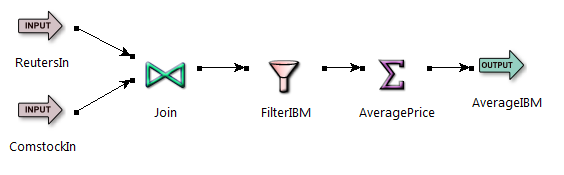
\includegraphics[width=\textwidth]{eventflow.png}
  \caption{This diagram represents a simple query where two streams
    are joined, non IBM tuples are filtered-out, and then the average
    of IBM stock prices over the last 5 minutes is sent to the
    output.}
  \label{fig:eventflow-sample}
\end{figure}

Some of the most important operators are:

\begin{description}
\item [Aggregate] Computes aggregate operations over windows of
  tuples. Supports the option to partition tuples into sets and then
  apply the aggregation over each individual set, much like a SQL
  GROUP BY statement;
\item [Filter] Discards some tuples from the input stream based on a
  predicate. Performs the same function as a SQL WHERE statement;
\item [Gather] Receives tuples from two or more streams and
  concatenates those with the same key. The resulting tuple values may
  be direct copies from the original tuples or the result of applying
  some expression to these;
\item [Join] Similar to SQL joins, this operator pairs tuples coming
  from two streams that match a given condition and outputs a new
  tuple whose fields may be specified by the user. In general, joining
  two infinite streams may require keeping all tuples from both
  streams in memory. To avoid problems later on, the user must specify
  timing constraints regarding matching tuples saying, for example,
  that they must arrive within 60 seconds of each other;
\item [Map] Similar to the first part of a SELECT statement, this
  operator transforms a tuple --- possibly discarding or adding new
  fields along the way ---, and sends it downstream;
\item [Pattern] Instructs the engine to look for specific patterns of
  events;
\item [Union] Acts as a multiplexer, connecting many input streams to
  a single output stream, to where all tuples are sent. Similar to the
  SQL UNION statement.
\end{description}

It's clear that most of these operators have SQL counterparts. There
are a few things that can be done in EventFlow but not in StreamSQL
(see the online documentation at \cite{eventflow2streamsql}), but
they're just small details, nothing that changes the developer's way
of thinking. It's then mostly a matter of taste --- not power ---, to
choose between StreamSQL and EventFlow.

\section{Oracle rules}
\label{sec:orm}

Oracle Rules Manager (ORM) \cite{orm:www} embraces a completely
different paradigm. Instead of writing queries, the user creates rules
that are made of three parts. The first, the event type, instructs the
system to trigger the rule only when an event of that type occurs. The
second, the condition, is a predicate that is compared against the
event. If they match, the third part, the action --- a PL/SQL
procedure ---, is executed.

Conceptually, a rule has the following format:

\lstset{
  language=Oracle,
  columns=fullflexible,
  basicstyle=\tt,
  keywordstyle=\bf,
}


\begin{lstlisting}
  on   <event>
  if   <condition>
  then <action>
\end{lstlisting}

The following example shows a simple rule:

\begin{lstlisting}
  on   StockTick(symbol, price)
  if   symbol = 'ACME' and price > 100
  then buyStocks(symbol)
\end{lstlisting}

The event shown above represents a stock update received from some
external source. These are the simplest kind of events, also called
\emph{primitive} events. ORM also supports \emph{composite} events
that are defined as combinations of other events. For example, it is
possible to define a composite event that occurs when ACME shares drop
10\% and, less than 5 minutes later, some other company's shares gain
2\%. To be more specific, the following types of combinations are
supported:
\begin{description}
\item [Sequencing] Specifies the order between events, i.e., event A
  must occur before event B;
\item [Negation] Checks for the non-occurrence of some event. Useful
  to raise exceptions when business rules are violated;
\item [Set semantics] Allows combining events with the AND operator to
  specify that all of them must occur for the composite event to occur
  as well;
\item [Any N] Checks for the occurrence of at least N children events;
\item [Collection] Combines a set of primitive events based on some
  common properties. Could be used, for example, to detect all
  costumers who withdrew more than \$1000 from their bank accounts
  during the past 24h.
\end{description}

ORM comes with a GUI utility to simplify the rules creation
process. This is necessary because creating a rule the hard way is a
daunting task that involves writing SQL queries containing XML blocks
containing SQL snippets inside. Still, there are situations when one
needs to avoid these utilities and work with real code, situations
where a simpler configuration process would be desirable.

The biggest disadvantage of rule-based languages comes from the
paradigm itself. While they may be effective for detecting complex
patterns of events, they are not so good when it comes to actually
processing the data. Built-in combinators provide some aggregation
functions, but these will seem basic for companies in need to
implement proprietary analysis algorithms. Also, PL/SQL is arguably
not a language suited for event-based complex application development.

One other issue that hinders these systems is the difficulty to reason
about their runtime behavior. As the number and complexity of rules
increases, an event may trigger more than one rule and these rules may
themselves trigger other rules, resulting in a cascading process that
may never end. This behavior makes the applications more difficult to
understand, to the point where even adding or removing a simple rule
may have unpredictable effects. These kinds of non-linear interactions
are discouraged by Software Engineering best-practices and thus, the
decision to use rule-based systems for building large applications
must be carefully pondered. To be fair, Oracle Rules Manager provides
constructs to deal with simultaneous triggering rules, but the problem
doesn't go away.

\section{Apama's MonitorScript}

When ESP solutions left the academia to meet the real world, many
users argued that SQL-based languages were ill-suited for many
information processing tasks. MonitorScript (MS) is Apama's response
to these complains.

Deriving from the procedural family of programming languages, MS
programs look a lot like Java programs. However, the most important
and unique feature it includes is the actor model based on having many
little \emph{processes} that execute in parallel and communicate with
each other through messages. In MS, these entities are called
\emph{monitors}. A monitor is an event processing agent that basically
sets up an arbitrary number of \emph{listeners} that await for the
occurrence of events. When one matching event arrives, monitors
process it. Monitors can also send events to each other, through the
\emph{route} statement.

Last but not least, monitors can have state. This means that instead
of writing a SQL query to capture the state of the system, MS updates
the state incrementally as the computation moves forward. The downside
is that, for simple things, SQL queries will definitely be easier to
understand, because a SQL query \emph{is} its intention while, in a
procedural program, the big picture is not always that clear.

To get a feeling for the language, here is a small MonitorScript
snippet:

\lstset{
  language=MonitorScript,
  columns=fullflexible,
  basicstyle=\tt,
  keywordstyle=[1]\bf,
  keywordstyle=[2]\it,
}


\begin{lstlisting}
monitor ProcessMarket {
    // Keep the last price per company
    dictionary <string, int> lastPerCompany;

    action onload {
        Tick tick;
        on all Tick(): tick {
           processTick(tick);
        }

        on all PriceRequest(): ev {
            processPriceRequest(ev);
        }
    }

    action processTick(Tick tick) {
        lastPerCompany[tick.sym] := tick.price;
        route TickAck(tick.sym);
    }

    action processPriceRequest(PriceRequest ev) {
        if (lastPerCompany.hasKey(ev.sym)) then {
            route PriceReply(ev.sym, lastPerCompany[ev.sym]);
        }
    }
}
\end{lstlisting}

This listing declares one monitor (\verb=ProcessMarket=), that waits
for \verb=Tick= and \tt Last- PriceRequest \rm events. When it receives a
new \verb=Tick= update, it keeps the price reported in a dictionary,
indexed by the company's symbol and replies with a \verb=TickAck=
message. When it receives a \verb=PriceRequest=, it fetches the last
price from the dictionary and sends a \verb=PriceReply= message.

Note the need to create request, reply and acknowledgment messages
when what one really wants to do is to perform a method invocation
between different monitors. Indeed, the runtime system could provide
some kind of remote procedure call mechanism and handle the low-level
details by itself.

MS and SQL are at opposite ends of the programming language
spectrum. While it simplifies a lot of tasks that don't naturally fit
into SQL, MS also looses all the querying capabilities that made SQL
and its derivatives popular for data processing.

\chapter{Simple questions, complex answers}
\label{chap:simple-questions-complex-answers}

In this chapter we are going to discuss some simple queries that are
very complex to express using existing SQL dialects for ESP
systems. We will try to understand the reasons for this difficulty and
propose solutions to eliminate it.

\section{Events are discrete, state is continuous}
\label{sec:acme-problem}

In the context of ESP applications, events are always discrete
entities, because they have a well defined position in time and the
information they carry becomes invalid outside that position. This
works for many scenarios that are discrete by nature --- earthquake
reports, orders placed in an online store, heart beats or even noise
readings sampled periodically, just to name a few. However, some
systems are truly continuous and the values reported by an event
influence what we know about the system and what we can conclude about
its state. Examples include price change reports, where we know that
the price of a product will remain the same until a later event
signals a change, temperature readings by a smart sensor that issues
reports only when the temperature differs by 0.1 degrees from the one
in the previous notification, or a goal scored in a football match
that updates its result until another goal is scored or the match
ends. Unfortunately, the semantics employed by ESP systems don't work
so well in these cases.

To see why, let's begin with a small example. Suppose we build an ESP
application to monitor noise-levels in a street, measured by a sensor
every 10 minutes. This application receives the following two events
and no others:

\begin{tabular}{ |l|r| }
  \hline
  Timestamp & Noise (dB) \\
  \hline
  11:00 am & 70 \\
  11:10 am & 50 \\
  \hline
\end{tabular}

Suppose further, that our application is interested in analyzing the
last 20 minutes of data and, to achieve that, uses a regular temporal
sliding window like the one discussed in section \ref{sec:sql}. Figure
\ref{fig:window-contents} shows the contents of this window between
11:00 am and 11:30 am.

\begin{figure}[htpb]
  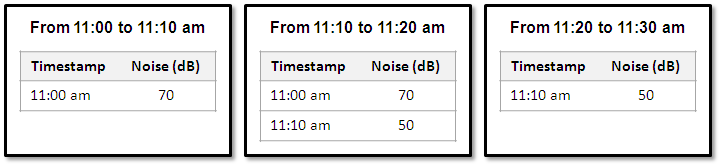
\includegraphics[width=\textwidth]{window-contents.png}
  \caption{Contents of the 20 minutes sliding window between 11:00 am
    and 11:30 am.}
  \label{fig:window-contents}
\end{figure}

By querying this window, we are now able to answer a few
questions. For example, at 11:10, the loudest reading registered
during the past 20 minutes was 70 dB, while 10 minutes later the
first event expires and the answer becomes 50 dB. Note that you cannot
ask for the loudest moment in the last 20 minutes, because a noisy
ambulance may have passed while the sensor was idle. That is, you
cannot assume anything in the time that goes from one event to
another. However, given the data that is available, the application
returns the correct answer.

This application is so successful that we are asked to adapt it to
monitor the stock market. Our clients are investors who want to be
able to make good decisions as quickly as possible and, to do so, our
application must handle events informing about every single
transaction. Suppose the application is deployed and receives the same
two events from the previous example, where instead of representing
noise-levels, they now refer to the value of ACME stock actions. Using
the same 20 minutes window, we may try to compute the highest price
attained by ACME during this period. At 11:10 am, the application will
return \$70, while at 11:20 am the answer will change to \$50, just
like in the previous example. However, this answer is known to be
wrong because the price remained at \$70 until 11:10 am and thus, the
answer should remain unchanged until 11:30 am\footnote{Strictly
  speaking, this is not how the stock market works: prices are not
  continuous and any investor may buy or sell for how much as he
  pleases. We ignore this detail because there are many situations --
  even in the stock market -- where it makes sense to treat discrete
  values as continuous.}. Despite using the same input data, posing
the same question and obtaining the same two results, one was correct
while the other was wrong.

\begin{figure}[h]
  \center
  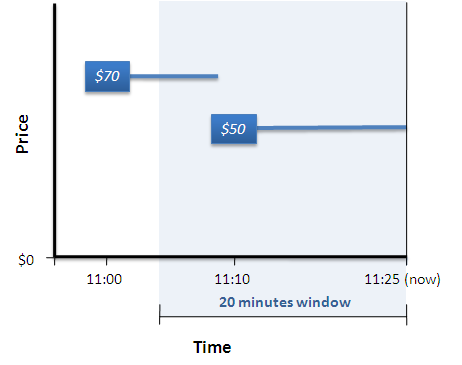
\includegraphics[width=0.7\textwidth]{outside-window.png}
  \caption{Evolution of ACME stock prices in the scenario described in
    the text. Values in boxes represent the two events received at
    11:00 am and 11:10 am. As you can see, at 11:25 am the first event
    lies outside the window and the engine will not consider it, even
    though its value remained valid throughout part of the window.}
  \label{fig:outside-window}
\end{figure}


The central difference between these two examples, pertains to what
can be assumed between events. There are three different cases:

\begin{itemize}
\item Between events the value is undefined. This is what happens when
  the value is discrete by nature --- the sender of a network packet
  is undefined when there is no network traffic ---, or when the event
  generator is sampling a continuous entity, like the noise sensor of
  the first example. We will refer to this as the \emph{pulse}
  semantics;
\item The value remains constant until the next event modifies
  it. This is valid if the value represents a new state, like the
  price of ACME stock actions, that remains the same between two
  updates. As such, we will call this the \emph{state-changes}
  semantics. Some continuous distributions that are known to be smooth
  may also be modeled under these semantics. For example, temperature
  may be assumed to remain constant between two updates, unless sudden
  variations not reported by the sensors are problematic;
\item In some rare cases, the value between events may be approximated
  by a well known mathematical function.
\end{itemize}

Existing languages adopted the pulse semantics by design. This is a
natural choice if we consider events as isolated occurrences. However,
if events represent changes in state, these languages will disappoint
because the developer has to manage this state manually. This can be
seen in Appendix \ref{sec:acme-problem-solution}, where a solution to
the ACME stocks problem, implemented in Coral8 CCL, is shown. The
algorithm creates two windows: the 20 minutes window and another
window that will contain the newest event older than 20 minutes (i.e.,
the event that most recently expired from the 20 minutes
window). Then, we perform a \verb=full outer join= between both
windows (\verb=union= would be more appropriate, but Coral8 doesn't
support it) and calculate the maximum price in either of them. As you
can see, this solution is quite verbose, which would be OK if only
there weren't so many situations like this, where the values are
continuous and must be handled with special care.

A slightly modified version of the ACME problem was posed on an online
community where researchers and vendors participate
\cite{simple-problem} \cite{simple-problem2}. It generated a lengthy
(more than 60 messages), interesting and sometimes funny
debate. Several vendors replied --- including Oracle, Aleri, Coral8
and Esper ---, and tried to find a good solution using their
products. In our opinion, they failed because their solutions were
verbose (like the Coral8 one above), inefficient or wrong. In the end,
some participants concluded this was not an event processing problem
anyway because it involves state and tried to dismiss it as
irrelevant, while others argued that queries like these show up every
day and if ESP engines can't solve them, their usefulness is reduced.

We agree that existing ESP engines shouldn't be applied to problems
like these, not because they don't matter, but because these engines
were not prepared to solve them --- even if they are able to do so
with more or less trouble. Instead, we believe these problems call for
a new language, encompassing both pulse and state-changes semantics,
that provides first-class constructs to deal with them.



\section{Defective products detection -- the ``too muggy'' query}
\label{sec:defective-products}

Another class of problems that are reasonable in the context of ESP,
but are difficult to solve by current systems, are those where the
developer needs to know for how long a certain condition was true (or
false). For example, imagine the following scenario, attributed to
Andrew Witkowski from Oracle and illustrated in figure
\ref{fig:factory}: a factory has several rooms, every room has at
least one humidity sensor and one temperature sensor. Furthermore,
products contain a RFID tag that is read by RFID sensors placed at the
entrance of each room. All these sensors send their readings to a DSMS
that needs to answer the following question: ``Which products stayed
more than 10 minutes (not necessarily consecutive) at more than 20
$^{\circ}$C and 80\% of humidity?''. These products are defective and
mustn't go to the shelves.

\begin{figure}[htbp]
  \center
  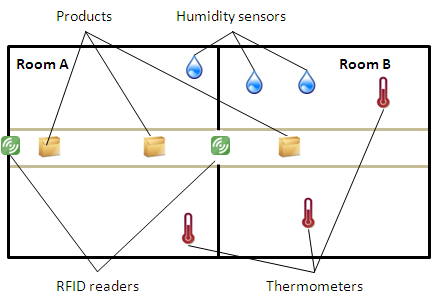
\includegraphics[width=0.6\textwidth]{factory.png}
  \caption{The factory outline.}
  \label{fig:factory}
\end{figure}


A solution for a simplification of this problem, written in Coral8
CCL, is shown in Appendix \ref{sec:defective-products-solution}. This
solution does not take humidity into consideration and assumes there
is only one sensor per room. The algorithm is simple: for each
product, we keep one counter with the time the product spent above 20
degrees, as well as the timestamp for when this counter was last
updated. When a product leaves a room, we update its counter if the
temperature in the previous room was higher than 20, and set the last
updated timestamp to the current time, given by the \verb=now()=
function. When the temperature changes, we do the same thing for all
products in that room.

This solution is quite long (3 pages of SQL-like code) as it is and it
still doesn't solve the original problem. Worse, the solution is long
and complicated because it needs much more than the standard operators
the language provides, which means that it is not possible to express
it using a few queries. Instead, the only way is resorting to an
algorithmic solution where the developer needs to explicitly write
down all the steps of the computation. This is, however, contrary to
the declarative nature of SQL and one has to wonder if using a
procedural language such as Python or Java -- where the developer is
able to create new operators better suited for the problem at hand --
wouldn't result in a simpler program. One may argue that this is a
difficult problem and the solution can't be simple
anyway. Nonetheless, it is a good exercise to analyze this piece of
code to see what else is wrong with it.

Let's begin by thinking about what would have to be modified to
support humidity. Naturally, we would have to create a new stream ---
\verb=hum_readings= --- that receives humidity readings from
sensors. Then, it would make sense to create a window to keep the last
humidity reading per room, analogous to the \verb=RoomTemperature=
window for temperatures. When the humidity changes, we need to
generate new events with the identifier of the room and its old
humidity, just like we do now when a product switches rooms or when
the temperature changes. When an event arrives in this stream, we
check if the previous humidity was greater than 80\% and if the
current temperature is above 20 degrees. If both conditions hold, we
may finally proceed to update the product's counter as well as its
last updated timestamp. Unfortunately, we are not done yet: it is also
necessary to modify the other queries, that are triggered when the
temperature changes or when the product switches rooms, to take the
current humidity level into consideration. Thus, adding new sensors
implies not only writing new queries, but also modifying existing
ones. Clearly, this approach does not scale\footnote{``scale'' here
  refers to the source code, not to the performance of the solution.}
as extensive rewrites are necessary every time the requirements are
modified. Software engineering best-practices dictate that, if
something like this happens, then the code is not modular enough or is
using the wrong abstractions.

The solution for this problem implemented in the appendix shows some
of these symptoms. There, besides the two input streams and the window
with the counter per product, we create two other windows and two
temporary streams. The windows contain the current and previous
temperatures of each room and the current and previous room for each
product. Thus, these windows are used to maintain the state of the
system. To support humidity, we would need a third window to maintain
the current and previous humidity level for each room. Note how
information (temperature and humidity) for a given entity (the room)
becomes scattered across several windows. To correlate temperature
with humidity, one would need to join these windows and then group by
the room's id. Thinking from an object-oriented point-of-view, it is
easy to see that this query would be greatly simplified if there was
some way to define \verb=Room= objects with properties such as
\verb=temperature= or \verb=humidity=, and use these objects in
queries, just like regular events. Moreover, one could instruct the
system to create the objects and manage their attributes
automatically, by looking at the right events. We could take this one
step further by supporting relationships between objects, akin to what
Object-Relational Mapping (O/RM) tools such as Hibernate
\cite{hibernate:www} do for regular databases. This way, each
\verb=Room= object would possess a list with its \verb=Product=s and
each \verb=Product= would include a reference to the \verb=Room= where
it is at. With these changes, finding the current temperature of the
room where a product is would be as simple as typing
\verb=product.room.temperature=.

% TODO: Make picture of the algorithm

As for the two temporary streams, their events are created when the
products switch rooms or when the temperature of a room changes, and
contain the previous room id or the previous temperature. These
streams are not strictly necessary as their code could be directly
inserted into the \verb=FROM= clause of the queries that use
them. However, this would not be a good idea as it would quickly
result in unreadable code. To avoid creating big and complex queries,
developers partition them into smaller ones connected by temporary
streams. Thus, streams end up being used as variables to store the
intermediate results of computations. But streams aren't a suitable
replacement for all kinds of variables. In procedural programming
languages, programmers can choose among primitive variables (int,
float, string, \dots), arrays, dictionaries, lists, sets and, why not,
objects. Certainly, streams and windows alone could be used to
simulate all these kinds of constructs, but they're just not the right
tool for \emph{every} job.

\section{Semantic windows}
\label{sec:semantic-windows}

Suppose that ACME stock is worth more than \$70 during some interval
and you want to know what was the average of its price during that
interval. Solving this problem using current technology is not so
difficult. Most ESP products include some kind of event detection
feature that allows the search for patterns of events. To obtain an
answer, we could find the event where ACME stocks passed the \$70
mark, then find all the events where the price stayed above that
threshold and, finally, find the event where they descended below
\$70. With all these events, we could then proceed to calculate the
average price.

There are two problems with this approach. The first is that the
detection of the boundaries of this interval may itself involve the
detection of another complex pattern. For example, to discover the
event where the price rose above \$70, one needs to compare some event
with the one that preceded it. The second problem is that these
complex event detection features work by first detecting the pattern
and then processing it. Thus, while the price remains above \$70, the
engine keeps all the events in memory and only when the price goes
below that mark will it proceed to calculating the average. This is
suboptimal, because the engine could keep a temporary sum of the
prices and a temporary count of the number of events received. These
two numbers are enough to generate the average and thus, the events
themselves could be discarded immediately.

A better way to solve this last problem is through \emph{semantic}
windows \cite{semantic-windows}. These are windows whose endpoints are
fixed by events, instead of being defined by time or number of
elements. Currently, no product supports this type of windows. Using
semantic windows we could instruct the engine to open the window when
the price ascends above \$70 and close it when it finally descends
below that mark. The advantage of this approach is that all windows
are closed eventually --- i.e., if the opening pattern is found, then
we are sure that there will be a corresponding closing event. Thus,
the engine knows a priori that there will be a successful match for
this window and may begin calculating the average right away, while
saving space by discarding the events that will be no longer needed.

Regarding the first problem --- detecting the moment the price passes
the threshold in either direction ---, notice that stock prices belong
to the state-changes class of problems discussed in section
\ref{sec:acme-problem}. Hence, the price evolution of ACME stocks may
be plotted using a continuous step-function over time, similar to the
one in figure \ref{fig:outside-window}. Our problem then becomes a
simple matter of cutting the plot horizontally where price equals 70,
ignoring the values below that value, and calculating the average for
the remaining plot. All of this could be done by the engine behind the
scenes, but only if it is smart enough to distinguish between pulse and
state-changes semantics.

\section{Summary}

In this chapter we have shown that there are problems where existing
languages perform poorly. We believe this happens because these
languages work at a very low level which forbids the developer to
think in terms of higher abstractions. In summary, the issues found
were:

\begin{itemize}
\item The pulse semantics, adopted by all engines, are unsuitable for
  many problems where the events represent state-changes of some kind;
\item It is difficult to decouple the various parts of a solution in
  such a way that introducing a new feature does not require rewriting
  part of the existing code;
\item Related data may be scattered across several streams and
  windows, forcing the developer to perform SQL operations --- in
  particular \verb=JOIN=s and \verb=GROUP BY=s ---, to join it
  together. We believe most of these queries could be made simpler by
  structuring the data in a different way, using objects;
\item In these languages, streams and windows are the only data
  structures available, while many algorithms would benefit from a wider
  choice;
\item Some problems require new operators -- semantic windows,
  operators to deal with time, new aggregators, etc -- but there is no
  way to create them.
\end{itemize}

It's not our purpose to claim that SQL, in general, is not well-suited
for ESP applications. However, we believe that ESP problems have their
own needs that require the availability of new data types, new
operators and different semantics, to the point where the resulting
language can hardly be called a SQL dialect anymore. Still, SQL has
benefits. For simple things, its declarative nature makes it very
expressive. Also, SQL querying capabilities are very powerful and
excel in many data processing tasks. It is understandable then, that a
new language should take some inspiration from SQL and borrow some
features to provide equally powerful constructs.

\chapter{A quick introduction to EzQL}
\label{chap:ezql}

In this chapter we introduce EzQL, our proposal to attack the issues
outlined in the previous chapter. Its main features are:

\begin{itemize}
\item The language integrates both pulse and state-changes semantics,
  discussed in the previous chapter. Thus, \emph{EzQL does not lose
    any ability offered by current systems}, while it also adds new
  capabilities;
\item Includes a simple modeling approach, akin to object-orientation,
  where real-world entities can be modeled as objects with properties
  --- temperature, price or speed, for example ---, whose values
  depend on the values of events. For instance, this entity-model
  allows the creation of many Room entities each with their own
  temperature attribute which is automatically updated as new sensor
  readings arrive. Furthermore, these entities and the values of their
  properties define the state of the application and this state can be
  queried just like regular events;
\item The entity model supports \emph{associations} between entities,
  inspired by Ob\-ject-Relational Mapping (O/RM) tools for
  databases. Thus, it is possible to say, for instance, that a room
  has many products and, correspondingly, that a product belongs to
  one room. Again, these associations may change as new events arrive,
  i.e., a product may leave one room and enter another. Naturally,
  these relationships can also be queried --- one can ask, for
  example, what is the cheapest product inside room A. This type of
  queries can already be written in currently available systems, but
  we will see that they become much simpler in EzQL;
\item EzQL tries to give more power to the developer, allowing him to
  create user-defined aggregators and functions. It also supports
  higher-order functions, an important medium to create new
  abstractions;
\item It comes with a static type-system supporting type-inference and
  parametric polymorphism. This increases the expressiveness of the
  language without loosing the capability to check and guarantee that
  programs are type-safe.
\end{itemize}


\lstset{
  language=EzQL,
  columns=fullflexible,
  basicstyle=\tt,
  keywordstyle=[1]\bf,
  keywordstyle=[2]\it,
  tabsize=8,
  showtabs=true,
  tab=$\hspace{1pt}$
}

\section{Streams and windows}
\label{sec:streams-windows}

As we will see, EzQL is very different from the query languages
presented in the state of the art. However, at its core, it still has
streams of events and operations to query them.

Suppose you are given a stream called \verb=stocks= that receives
events from the financial market. These events contain three fields --
\verb=timestamp=, \verb=symbol= -- which is the company id --, and
\verb=price=. In EzQL you would start by declaring this stream with:

\begin{lstlisting}
  stocks = stream of { timestamp:int, symbol:string, price:float }
\end{lstlisting}

Now, the stream is ready to be used and you may query its data. For
example, to multiply the price of ACME events by two, you could write:

\begin{lstlisting}
  acmeStocks_x2 =
    from ev in stocks			# For each event ev in the stream
    where ev.symbol == "ACME"
    select { price_x2 = ev.price * 2 }
\end{lstlisting}

The syntax is inspired in SQL and that is only natural, as SQL handles
these simple queries very well. The only bit that deserves some
explanation is the segment between braces after \verb=select=. This
creates an event with one field -- \verb=price_x2= --, which we define
as twice the price held by the original event. The \verb=select=
operator implicitly adds a second field to the event -- the
\verb=timestamp= --, which is copied from the original event being
projected.

The result of this operation is a new stream --
\verb=acmeStocks_x2=. The next listing shows off a few more features
that EzQL shares with other languages, namely temporal windows and
aggregations:

\begin{lstlisting}
  avg_5min =
    let cheapStocks =
      from ev in stocks[5 min] 	 # For each event in the 5 min window
      where ev.price < 20
    cheapStocks.avg (:price)
\end{lstlisting}

This example computes the average price of all events received during
the last 5 minutes where the price is under \$20. The query has been
partitioned into two smaller sub-queries: the first --
\verb=cheapStocks= --, is a local variable declared using \verb=let=
that contains a stream with the filtered events, and the second is the
application of the \verb=avg()= method over \verb=cheapStocks=. To
understand this query, the reader should know that, in EzQL as in
other languages such as Python, indentation is significant. This
means that instead of using \verb=begin= and \verb=end= or \verb={=
  and \verb=}= to denote code blocks, we simply align related
statements using whitespace.

The resulting number is stored in \verb=avg_5min= and we may use it in
other queries. For example, to check if the average is smaller than 10
we could write:

\begin{lstlisting}
  isSmall = avg_5min < 10	# This is a query!
\end{lstlisting}

While it may seem uninteresting, this example illustrates one
important point that is essential to understand EzQL: \verb=isSmall=
is a continuously running query. Every time the average price changes,
the number stored in \verb=avg_5min= is updated, which then triggers
the re-computation of \verb=isSmall=. The engine works like a
spread-sheet application where a modification to one cell is
automatically propagated to other cells that depend on the first, and
so on.

\section{Continuous values}
\label{sec:continuous-values}

This example also shows the first major difference between EzQL and
other ESP languages: in EzQL, the result of an aggregator such as
\verb=avg()= is a continuous number and not a stream where events are
sporadically sent to every time the aggregated value changes. These
numbers are part of a large family of data types that we call
continuous values. The rationale behind the decision to introduce
continuous values instead of reusing streams is that, as we have seen
in chapter \ref{chap:simple-questions-complex-answers}, events are
ephemeral -- they come and, in the next instant, they are
gone. However, the maximum price over the last five minutes, for
example, will remain the same until a greater price arrives or the
current one expires. So, it makes sense to treat the maximum as a
continuous entity, whose value is always defined. However, in
traditional languages, if we need the current maximum at any time, we
must keep it inside a window with a single entry created specifically
for this purpose. We believe this represents an undesired level of
indirection that impacts the amount of code that needs to be written
and hides its meaning. It feels unnecessary to create a window when a
simple number would suffice. Thus, continuous values were born.

They are not restricted to numbers, though. For example,
\verb=isSmall= declared above is a continuous boolean that alternates
between \verb=true= and \verb=false=. All the other data types EzQL
supports (that we have yet to discuss) -- strings, records, tuples,
enumerations, closures, entities and dictionaries --, may be treated
as continuous entities.

Besides aggregators, the other primary operator that creates
continuous values is \verb=last()=. Conceptually, \verb=last()= works
by taking a stream that produces events and \emph{holding} each event
in sequence, until the arrival of the following event makes it
obsolete. Figure \ref{fig:last} illustrates this. This operator is
useful in many situations where the \emph{last} event defines the
\emph{current} state of the system. For example, an application that
manages financial data using the \verb=stocks= stream may consider the
current price of some company's stocks the same as the price that came
in the last event related to that company. According to this line of
reasoning, the current price of ACME could be found with:

\begin{figure}[t]
  \centering
  \subfloat[A regular stream.]{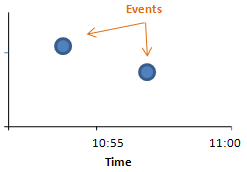
\includegraphics[width=0.4\textwidth]{last-a.png}}
  \subfloat[The same stream, after applying \tt last() \rm to hold its events.]{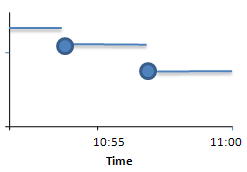
\includegraphics[width=0.4\textwidth]{last-b.png}}
  \caption{How \tt last() \rm works.}
  \label{fig:last}
\end{figure}


\begin{lstlisting}
  acmePrice =
    let acmeStocks =
      from ev in stocks
      where ev.symbol == "ACME"
    acmeStocks.last().price	 # Get the price from the last event
\end{lstlisting}

All continuous values may change as time passes or new events
arrive. As discussed, the system takes care of spreading these changes
automatically and transparently. However, in the same way that we can
create a window to analyze past events, we may also exploit the
temporal information contained in continuous values. As such, it is
possible to open windows and apply aggregators over regular integers,
booleans or other values. The following listing illustrates this:

\begin{lstlisting}
  maxAcme_1h = acmePrice[1 hour].max()
\end{lstlisting}

This results in the maximum price ACME's stocks attained over the
course of the last hour. Note that the 1 hour window is created over
\verb=acmePrice= -- that is, the continuous value that holds the
current price. You could have solved this by opening a regular event
window over the stream that contains only ACME's events:

\begin{lstlisting}
  maxAcme_1h_wrong =
    let acmeStocks =
      from ev in stocks
      where ev.symbol == "ACME"
    acmeStocks[1 hour].max(:price)
\end{lstlisting}

Surprisingly though, the results would differ. To see why, note that
this is just another instance of the pulse vs state-changes problem
discussed in section \ref{sec:acme-problem}: the price could have been
at its maximum 1 hour ago, but the notification for this value might
have happened a little earlier and thus, a regular sliding window
applied to a stream would not consider it when calculating the
maximum. A continuous value, on the other hand, retains its value
until a new event changes it. Thus, querying \verb=acmePrice= for its
maximum value over the last hour would consider all the values it had
during that time --- even if the corresponding event came earlier ---
and would give the correct result.

\begin{figure}[t]
  \centering
  \subfloat[maxAcme\_1h\_wrong]{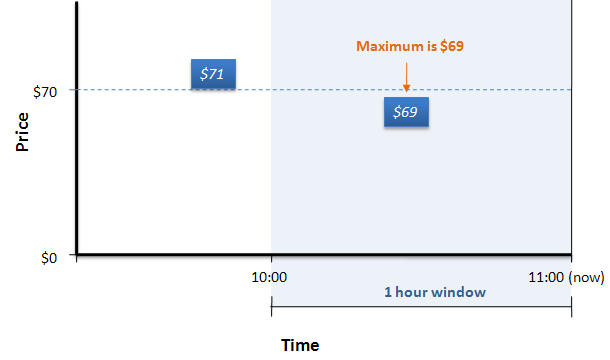
\includegraphics[width=0.5\textwidth]{maxAcme-wrong.png}}
  \subfloat[maxAcme\_1h]{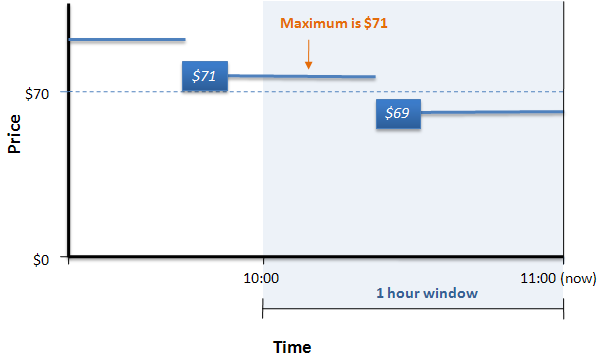
\includegraphics[width=0.5\textwidth]{maxAcme.png}}
  \caption{In the first case, the maximum is \$69 because only the
    second event lies inside the window. In the second, though, a
    continuous value is used to hold the higher price so that it still
    belongs to the window.}
  \label{fig:acme}
\end{figure}


% TODO Imagem a ilustrar a diferença

This is surprising because continuous values were introduced to
simplify queries and because they ``kind-of make sense''. Nonetheless,
they also introduce state and this seemingly innocuous change has
profound implications. Through them, we can now support the
state-changes semantics discussed in chapter
\ref{chap:simple-questions-complex-answers} while retaining support
for pulse semantics by using regular stream operations.

The counterpart of \verb=last()= is \verb=changes()=. This operator is
applied to a continuous value and results in a stream that receives
events every time the continuous value changes. These events have two
fields: \verb=timestamp= -- the timestamp of the change --, and
\verb=value= -- the new value. Applying \verb=last()= on
\verb=changes()= gets the continuous value back. That is,

\begin{lstlisting}
  v <=> v.changes().last().value
\end{lstlisting}

Continuous values are a natural medium to express a few recurring
patterns. For example, a common problem in ESP asks if a given
condition was true any time or every time during some period of
time. In EzQL, this can be done with the \verb=any?()= or
\verb=all?()=\footnote{EzQL allows functions that end in '?'; a
  convention, found in other languages such as Scheme and Ruby, that
  indicates that the function is a predicate.}  aggregators:

\begin{lstlisting}
  isSmall = maxAcme_1h < 20

  alwaysSmall = isSmall[1 hour].all?()
\end{lstlisting}

In the previous example, \verb=isSmall= is a boolean value that is
true if the maximum price over the last hour for ACME is smaller than
\$20. Since this maximum will vary, \verb=isSmall= is expected to
alternate between \verb=true= and \verb=false=. To check if the
maximum was always small, we just need to open a 1 hour window over
\verb=isSmall= and use \verb=all?()= over that window.

A related problem asks for the duration of a given condition. In EzQL,
we can solve it using the \verb=howLong()= aggregator\footnote{50 min
  means 50 minutes}

\begin{lstlisting}
  mostlySmall = isSmall[1 hour].howLong() > 50 min
\end{lstlisting}

\section{Dictionaries}
\label{sec:dictionaries}
The next example shows how to obtain the current price per company:

\begin{lstlisting}
  pricePerCompany =
    from stocks
    group by :symbol into events
    select events.last().price
\end{lstlisting}

\verb=group by= works by partitioning the events from the input stream
into N smaller streams, one per group. In the example above, each one
of these streams is given the name \verb=events= and then, for each
one in parallel, the price from its last event is retrieved -- using
the \verb=last()= method --, to be used as the resulting value of the
query. Note that we don't declare a variable to hold the event -- as
in \verb=from ev in stocks= --, because we don't need the event for
the remaining expression.

In this listing, \verb=pricePerCompany= is a dictionary that maps keys
(the company symbols) to values (the current price of their
stocks). Moreover, being the result of a continuous query,
\verb=pricePerCompany= is also a continuous entity: when a new event
arrives, the price of its company is automatically updated and every
time a previously unseen symbol is processed, a new entry is created
for it. Moreover, these changes are automatically propagated to other
queries that depend on them, as can be seen in the next example:

\begin{lstlisting}
  cheapCompanies =
    from price in pricePerCompany
    where price < 20
    select price
\end{lstlisting}

\verb=cheapCompanies= is a filtered dictionary: it contains only those
companies whose current price is under \$20. Every time a company goes
above this threshold, it is removed from the dictionary; and every
time the stocks of some company descend below \$20, a new entry is
created for it.

Sometimes one needs to return multiple values in the same query. For
example, one might need to return the maximum and average prices over
the last 5 minutes for all companies. In EzQL, this can be done as
follows:

\begin{lstlisting}
  avgMax_5min =
    from stocks
    group by :symbol into events
    select
      let ev5 = events[5 min]
      { maximum = ev5.max(:price), average = ev5.avg(:price) }
\end{lstlisting}

Note that there is no \verb=select let= operator: we are simply
declaring the local variable \verb=ev5= inside the \verb=select='s
projector, because we will need its value twice. The segment in braces
creates a record with two attributes: \verb=maximum= and
\verb=average=. One can access individual attributes in a record using
the dot (\verb=.=) operator. For example, it is possible to access
ACME's maximum price with:

\begin{lstlisting}
  acme_max = avgMax_5min["ACME"].maximum
\end{lstlisting}

This example also shows how to index individual entries inside a
dictionary using square brackets. Whenever a new event is received for
ACME, or an old event leaves the 5 minutes window, \verb=acme_max=
will automatically be updated to reflect this change.

To conclude this section, we show how to perform aggregations over
dictionaries. For example, to find the company with the cheapest
stocks overall, you could write:

\begin{lstlisting}
  cheapest =
    let companies =
      from stocks
      group by :symbol into events
      select events.last()
    companies.values().minBy(:price).symbol
\end{lstlisting}

\verb=companies= is a dictionary that contains the last event received
for each company. Remember that a dictionary maps keys to values. The
method \verb=values()= allows us to obtain a list containing just the
values which, in this case, are the events. To this list, we apply the
\verb=minBy()= aggregator which returns the event with the lowest
price. Finally, we access the \verb=symbol= field of this event to
obtain the corresponding company id.


\section{Modeling entities}
\label{sec:entities}

\subsection{Motivation}

In chapter \ref{chap:simple-questions-complex-answers}, we argued that
some queries would become simpler if the developer could model the
state of each entity and the relationships between them using
objects. In this section we will explain how to do this in EzQL using
a simple fictional scenario based on a factory. This factory has many
rooms and each room is crossed by a pipeline that carries products
between rooms. Furthermore, each room has one temperature sensor --
because the conditions under which the products are manufactured must
be rigorously controlled --, and one RFID sensor that signals the
entry of a new product in the room. We can model this scenario using
two streams:

\begin{itemize}
\item
  \verb!tempReadings = stream of { roomId:string, temperature:float }! \linebreak which receives temperature readings per room;
\item \verb!entries = stream of { roomId:string, productId:int }! \linebreak whose events are
  created when a product has entered a room.
\end{itemize}

For this particular use-case, it might be appropriate to keep all
room's and product's data in two dictionaries:

\begin{lstlisting}
  # For each room, gather its current temperature
  allRooms =
    from tempReadings
    group by :roomId into events
    select
      let ev = events.last()
      { roomId = ev.roomId, temperature = ev.temperature }

  # For each product, gather the id of its current room
  allProducts =
    from entries
    group by :productId into events
    select
      let ev = events.last()
      { productId = ev.productId, roomId = ev.roomId }
\end{lstlisting}

With these dictionaries we can, for example, find out which products
are in rooms where the temperature is greater than 30 degrees:

\pagebreak
\begin{lstlisting}
  hotProducts =
    from p in allProducts
    where allRooms[p.roomId].temperature > 30
    select p
\end{lstlisting}

Or how many products are in each room:

\begin{lstlisting}
  productsPerRoom =
    from r in allRooms
    select
      let prodsInR =
        from p in allProducts
        where p.roomId == r.roomId
      prodsInR.count()
\end{lstlisting}

While this approach works, it also feels rather unnatural. Basically,
\verb=allRooms= and \verb=allProducts= are nothing more than
containers for the current state of all rooms and products known by
the system. This current state is very easy to manage and if you look
closer at their queries, you'll see that they have a lot in common:
the only things that change are the attribute names. Furthermore, the
queries for \verb=hotProducts= and \verb=productsPerRoom= follow
directly from the fact that there is an association between rooms and
products: at any given moment, a product is in one room while each
room may contain any number of products. As a consequence, these
queries also exhibit a few common patterns that should be abstracted.

\subsection{Modeling simple entities}

To improve this situation, EzQL includes an entity framework inspired
by Object-Relational Mapping tools for databases, that allows the
developer to model the entities that make up a scenario, as well as
the associations between them. Entities may be seen as streamlined
versions of classes in OOP programming created with event processing
in mind. This results in simpler queries compared to the ones
above. For example, defining an entity to model rooms can be done as
follows:

\begin{lstlisting}
  entity Room =
    createFrom (tempReadings, :roomId)
\end{lstlisting}

This declares an entity named \verb=Room=. The core of this definition
is the \verb=createFrom= operator that instructs the system to
automatically create new \verb=Room= instances whenever a previously
unseen \verb=roomId= arrives on \verb=tempReadings=. In addition,
\verb=createFrom= adds the stream fields to the entity. This way,
every \verb=Room= ends up with two attributes: \verb=roomId= and
\verb=temperature=. These attributes are continuous values, which
means they are automatically filled and updated by the system as new
events arrive. \verb=createFrom= adds one final member to all
entities, which is the stream \verb=events= we have been using in
examples with \verb=group by=. This stream contains all events that
are related to that particular entity. For example, in the listing
above, the \verb=events= field for room A would countain all events in
tempReadings where the \verb=roomId= field is "A".

Having declared \verb=Room=, we can now run a simulation to see how
the system manages these entities automatically. All the \verb=Room=
instances are accessible using \verb=Room.all=. This is a dictionary
that maps \verb=Room= id's (taken from the \verb=roomId= field in
this case) to the \verb=Room=s themselves. In essence, it plays a similar
role to \verb=allRooms= above. If the stream \verb=tempsReadings=
receives the following events:

\begin{tabular}{ |l|l|c| }
  \hline
  \verb=timestamp= & \verb=roomId= & \verb=temperature= \\
  \hline
  11:00:00 am & \verb="A"= & 20 \\
  11:01:00 am & \verb="B"= & 29 \\
  11:02:00 am & \verb="A"= & 23 \\
  11:03:00 am & \verb="B"= & 30 \\
  \hline
\end{tabular}

then \verb=Room.all=, if evaluated after 11:03:00 am, will return:

\begin{tabular}{ |l|l| }
  \hline
  Entity id & Entity \\
  \hline
  \verb="A"= & Room with roomId = \verb="A"=, temperature = 23 \\
  \verb="B"= & Room with roomId = \verb="B"=, temperature = 30 \\
  \hline
\end{tabular}

Naturally, we can query these entities as if they were normal streams:

\begin{lstlisting}
  hotRooms =
    from   room in Room.all		# For all rooms...
    where  room.temperature > 25
    select room.roomId
\end{lstlisting}

This results in a subset of \verb=Room.all= containing only one room:

\begin{tabular}{ |l|l| }
  \hline
  Entity id & Entity \\
  \hline
  \verb="B"= & Room with room\_id = \verb="B"=, temperature = 30 \\
  \hline
\end{tabular}

\subsection{Modeling associations}
\label{sub:associations}

Modeling associations between entities is just as easy. For instance,
to specify the one-to-many relationship between products and rooms we
may redefine the entities as follows:

\begin{lstlisting}
  entity Room =
    createFrom (tempReadings, :roomId)
    hasMany :products


  entity Product =
    createFrom (entries, :productId)
    belongsTo :room
\end{lstlisting}

The \verb=hasMany= annotation adds an implicit \verb=products= field
to the \verb=Room= entity. This field is a dictionary with all the
\verb=Product= instances that are in each \verb=Room=. Its definition
is equivalent to:

\begin{lstlisting}
  products =
    from p in Product.all
    where p.roomId = <roomId>
\end{lstlisting}

We can apply other dictionary operators to this attribute. To show
this, the next example finds which products that are now in room A
were also in room B less than 5 minutes ago:

\begin{lstlisting}
  from p in Room.all["A"].products
  where (p.roomId == "B")[5 min].any?()
\end{lstlisting}

Given that \verb=p.roomId= is a continuous value, so is its comparison
with ``B''. Therefore, we may open a temporal window to obtain the
results of this comparison over the last 5 minutes, to which we then
apply the \verb=.any?()= aggregator to check if the value was true any
time during that interval. If it isn't, \verb=where= will filter out
the product from the resulting dictionary. This example also features
a previously unseen situation where the predicate requires historical
data in order to actuate. This poses some difficulties because the set
of products that are in room A is constantly changing and, in order to
work correctly, the system must take that into consideration. That is,
as soon as a product arrives into room A, its 5 minute data must
already be available. The implementation of this class of queries --
that combine filtered dictionaries with temporal windows -- presents
some challenges that will be discussed in chapter
\ref{chap:implementation}.

Proceeding with the previous example, \verb=belongsTo= sets up the
reverse association, i.e., every product is inside one room. Moreover,
this instruction also adds an attribute \verb=room= to every
\verb=Product=. Thus, you could find which room product 123 is in
with:

\begin{lstlisting}
  Products.all[123].room
\end{lstlisting}

This may seem like a bit of hidden magic at first, but it's really
just a simple convention\footnote{This convention was inspired from
  the Ruby on Rails web framework \cite{ror:www}.}:

\begin{enumerate}
\item The \verb=:products= parameter to \verb=hasMany= instructs the
  engine to create a list of \verb=Product= instances. It knows that
  this list should hold \verb=Product=s, because ``product'' is the
  singular of ``products''. This list will be named \verb=products=;
\item On the other hand, the \verb=:room= parameter to
  \verb=belongsTo= tells the engine to create a field named
  \verb=room= in every product. This field will hold an instance of
  the \verb=Room= class (once again, it finds the class name through
  the parameter);
\item The engine fills the \verb=room= attribute of every product by
  checking its \verb=roomId= field. Remember, this field was created
  automatically by \verb=createFrom=. Given the identifier of the
  room, the engine can easily look up the corresponding \verb=Room=
  instance using the \verb=Room.all= dictionary;
\item The \verb=products= list in every \verb=Room= is filled using
  the reverse relationship. That is, the products that belong to room
  A are those where the condition \verb!room_id == "A"! is true.
\end{enumerate}

\subsection{Defining additional attributes}

It is possible to define new attributes on top of those that are
created automatically by \verb=createFrom=, \verb=hasMany= and
\verb=belongsTo=. For example, suppose we want to add a
\verb=temperature= attribute to every product that is taken from the
temperature of the room where the product currently is. We could do it
with:

\begin{lstlisting}
  entity Product =
    createFrom (entries, :productId)
    belongsTo :room

    # 'this' represents the current instance, as in Java.
    member this.temperature = this.room.temperature

\end{lstlisting}

There is a subtle detail in this definition: despite being equal to
the temperature of the current room, the product's temperature has a
``life of its own'' when it comes to history. That is, the past values
of the product's temperature reflect the fact that the product might
have been in other rooms. Hence, \verb=this.room.temperature[5 min]=
is, in general, different from the current room's temperature over the
last 5 minutes.

\section{When blocks}

Event processing problems are all about executing the right actions
when something happens, be it the arrival of a new event or the
expiration of an old one. In EzQL, we decided to abstract the notion
of \emph{when} to execute an action as much as possible, because this
results in queries that are more declarative and less
algorithmic.\footnote{If you're not convinced about this, go back to
  the previous section, choose any query, and try to enumerate the
  external events that, ultimately, trigger the re-evaluation of the
  entire query}. Allowing the developer to write his queries in a
higher-level of abstraction, without needing to worry about such
details (``What happens if two events arrive at the same time?'',
``What happens if, at the same time, an event expires and another
arrives at a window?'')  should be seen as one of the most important
features of EzQL.

Nonetheless, there are situations where specifying the right time to
execute some action is actually the way to go. It gives the developer
more freedom and allows him to do things that couldn't be done using
the standard operators. For example -- and continuing with our rooms
and products example --, suppose you'd like to know, for each room,
how many products entered the room, but only if the room's temperature
was hot (greater than 25). In EzQL you could employ \emph{when blocks}
to solve this problem:

\begin{lstlisting}
  entity Room =
    createFrom (tempReadings, :roomId)
    hasMany :products

    member this.hotEntries = 0
      # When there is an event in the 'entries' stream
      when ev in entries ->
        # If the entry happened in this room and this room is hot...
        if ev.roomId == this.roomId and this.temperature > 25
          then this.hotEntries + 1
          else this.hotEntries


\end{lstlisting}

The snippet above adds a new field called \verb=hotEntries= to the
\verb=Room= entity. When a room instance is created, this field starts
at 0. However, when a product enters a hot room (signaled by
\verb=when ev in entries -> ...=), the \verb=hotEntries= field for the
corresponding room instance will be incremented by 1, while all the
other rooms will remain unchanged.

You may also use when blocks with more than one stream. For example,
resetting the \verb=HotEntries= counter when the temperature goes below
25 is a straightforward extension:

\begin{lstlisting}
    member this.hotEntries = 0
      when
        | ev in entries ->
            if ev.roomId == this.roomId and this.temperature > 25
              then this.hotEntries + 1
              else this.hotEntries
        | this.temperature.changes() if this.temperature < 25 -> 0
\end{lstlisting}

In this example there are two paths that may be followed -- one when
there is an entry and the other when the temperature changes. We make
this choice explicit by including the pipe (\verb=|=) operator next to
each path. The \verb=changes()= operator was introduced in section
\ref{sec:continuous-values}. Basically, it converts the attribute
\verb=this.temperature= into a stream with the different values it
takes during execution. When an event arrives into that stream
(meaning: when the temperature changes), if the new temperature is
below 25, then \verb=hotEntries= will be reset to 0. Notice that
\verb=ev in...= is optional: if the event itself is not necessary,
there is no need to declare it.

The careful reader will notice that these last two examples are the
perfect testbed for a feature that was proposed in section
\ref{sec:semantic-windows}: semantic windows. EzQL does not provide
lexical support for these constructs. Yet, as we can see, when blocks
already come with the power necessary to solve the same
problems. Maybe the syntax could be improved, but it's not like when
blocks are difficult to use. Besides, modifying the syntax is the easy
part.

\section{Enumerations and pattern matching}
\label{sec:enumerations}

Sometimes we would like to classify the status of a set of entities
using descriptive names. For example, a room could be categorized as
hot or cold, crowded or empty. We could use strings for this, but
strings are not type-safe (what happens if the programmer makes a
typo?). Enumerations and pattern matching are two features commonly
found in functional languages that work together to help solve these
problems.

Conceptually, an enumeration is a value that may take a number of
forms. For example, an enumeration to classify the room temperature
may be declared with:

\begin{lstlisting}
  enum RoomState =
    | Cold
    | Hot
\end{lstlisting}

We could now define a \verb=state= attribute inside the definition of
the \verb=Room= entity that classifies the room as cold or hot:

\begin{lstlisting}
  member this.state =
    if this.temperature <= 25
      then Cold ()
      else Hot ()
\end{lstlisting}

You need to add \verb=()= because, in this context, \verb=Cold= is a
kind-of constructor that creates \verb=RoomState= instances
initialized to the \verb=Cold= state. Below, we will show how to pass
parameters to these constructors. Now, to find out how many rooms are
hot we could write the following query:

\begin{lstlisting}
  hotCount =
    let hotRooms =
      from room in Room.all
      where room.state == Hot ()
    hotRooms.count()
\end{lstlisting}

Enumerations may also carry payloads -- i.e., each state may also
include inner state. For example, suppose that we want to know how
many products entered the room while it was hot. This is the exact
same problem that we solved in the previous section, but we are now
going to present an alternative solution. First, let's add a counter
to the hot state:

\begin{lstlisting}
  enum RoomState =
    | Cold
    | Hot of int  # int is the type of the counter
\end{lstlisting}

Now we need to manage this counter inside the definition of the
\verb=state= attribute:

\begin{lstlisting}
  # Is this room hot or cold?
  member this.isHot = this.temperature > 25

  member this.state = null
    when
      | (this.isHot).changes() -> if this.isHot then Hot (0) else Cold ()
      | ev in entries if ev.roomId == this.roomId ->
          match this.state with
          | Cold -> Cold ()
          | Hot c -> Hot (c + 1)

\end{lstlisting}

%% TODO: Talk about NULL before

The first part of this definition is straightforward: the initial
value is \verb=null= -- because we don't know if the room is hot or
cold in the beginning --, and we alternate between the \verb=Hot= and
\verb=Cold= states when the \verb=isHot= condition changes. Notice
that we pass \verb=0= to the \verb=Hot= state, to initialize the
counter.

In the second part we use pattern matching for the first time. The
\verb=match ... with= operator provides a way to deconstruct an
enumeration. Basically, if the current value is \verb=Cold=, the next
value will continue to be \verb=Cold=. However, if the current state
is \verb=Hot c= for any counter \verb=c=, then we would like the next
state to be \verb=Hot= with the counter incremented by one.

Now we may use these definitions to find out how many rooms are
\verb=Hot= and have more than 10 entries at the same time:

\begin{lstlisting}
  hotPopulatedCount =
    let hotRooms =
      from room in Room.all
      where match room.state with
              | Hot c if c > 10 -> true
              | _ -> false
    hotRooms.count()
\end{lstlisting}

Inside \verb=match ... with=, the underscore means ``match anything''.

Arguably, this might not be the best example to illustrate the full
potential of enumerations and pattern matching. After all, we could
have done the same using the concepts from the last section -- and the
result would probably have been easier. However, the purpose of this
section is to introduce the reader to these new concepts. The real
usefulness of enumerations and pattern matching will be demonstrated
in the next chapters.

\section{Functions}
\label{sec:functions}

EzQL allows the developer to create user-defined functions and use
them in queries. The following example implements the factorial
function and uses it to calculate the factorial of the number of
products in room A:

\begin{lstlisting}
  def fact n =
    if n == 0
      then 1
      else n * fact (n - 1)

  factCount = fact (Room.all["A"].products.count())
\end{lstlisting}

When the number of products inside the room changes, the system
automatically reevaluates the entire expression and updates
\verb=factCount=.

In EzQL, functions are not static. Quite the contrary, functions are
allowed to change and their modifications are propagated downward to
the places where they are used. The best way to illustrate this is
through an example:

\begin{lstlisting}
  def twoHourMax id =
    let prodCount = Room.all[id].products.count()
    prodCount[2 hour].max()

  maxProductsPerRoom_2h =
    from room in Room.all
    select twoHourMax (room.roomId)
\end{lstlisting}

This snippet calculates the maximum number of products that were in
each room over the past two hours. To avoid duplication, the code
responsible for this calculation has been abstracted inside a function
-- \verb=twoHourMax= --, that receives the id of the room as a
parameter. The function itself depends on the result of the
\verb=count()=. When \verb=prodCount= changes, the entire body must be
reevaluated, because a new maximum may have been found and we want
\verb=maxProductsPerRoom_2h= to be immediately updated. Furthermore,
the function includes a kind of internal state -- the 2 hours window
--, that may itself trigger the computation of a new value.

The next example combines functions with when blocks to illustrate the
full potential of treating functions as active entities:

\begin{lstlisting}
def sumValues (n:int) =
  let acc = 0
    when n.changes() -> acc + n
  acc
\end{lstlisting}

The function \verb=sumValues()= receives an integer\footnote{Type
  declarations are optional in EzQL. In this example we declared n as
  an integer for documentation purposes only. If we had omitted this
  declaration, the system would have inferred it anyway.}. Inside the
body, we declare a variable -- \verb=acc=, that will act as an
accumulator. \verb=acc= starts at 0 and then, when \verb=n= changes,
it sums the new \verb=n= into the old \verb=acc=. In practice,
\verb=sumValues()= is equivalent to the built-in \verb=sum()= method
for integers. That is, \verb=Room.all.count().sum()= and
\verb=sumValues (Room.all.count())= would return the same result.

This example showed how functions can be used to implement
user-defined aggregators (UDA). We believe this is an important
feature, because many programs require aggregations that go beyond the
usual \verb=min=, \verb=max=, \verb=avg=, \verb=sum= and
\verb=count=. Chapter \ref{chap:eval} will explore this idea with a
few more examples.

\section{Additional features}

EzQL supports a few other features that are commonly found in other
general-purpose programming languages. Two of them are of particular
importance and deserve to be mentioned: higher-order programming and
the type system.

\subsection{Higher-order programming}
\label{sec:higherorder-programming}

Higher-order programming is a style where functions are treated as
regular values like strings or integers, and may be passed as
parameters, assigned to variables, created dynamically much like one
creates a string on runtime, returned from functions, etc. The idea
comes from the lambda calculus \cite{tapl} -- a mathematical
abstraction developed by Alonzo Church equivalent in power to Turing
Machines, that is at the core of programming language theory. It has
influenced the design of dozens of programming languages, most notably
the ones from the functional paradigm. Higher-order programming is
hailed as one of the most important ways to create new abstractions
that allow a language to grow and adapt to new problems without
modifying its syntax or compiler. Entire books on this topic have been
written and thus, describing it in any detail is out of scope of this
text. The interested reader may want to get a copy of \cite{sicp},
which is perhaps the best book on the subject ever written.

% If you have been reading this chapter carefully, you might have
% noticed that EzQL does not support loops. This is because we may use
% higher-order functions to simulate them, which means that there is no
% need -- EzQL being a research language -- to provide special syntax
% for them. The following example implements a simple iterator that
% loops from \verb=start= to \verb=end= and calls \verb=body= -- which
% is a function -- every iteration, passing the current counter as a
% parameter:

% \begin{lstlisting}
%   def for (start, end, body) =
%     if start <= end then
%       body (start) # Call the body
%       for (start + 1, end, body) # Increment and iterate again.
% \end{lstlisting}

% We could use \verb=for= to print all the rooms in \verb=Room.all= to
% the screen:

% \begin{lstlisting}
%   for (0, Room.all.count() - 1,
%     fun i -> print (Room.all.values()[i]))
% \end{lstlisting}

% The third argument -- \verb=fun i -> ...= --, is an anonymous function
% that receives one parameter \verb=i= and prints the \verb=Room= at
% index \verb=i=.

\subsection{Type system}
\label{sec:type-system}

A type system is a sub-component of most programming languages whose
main task is to prove the absence of certain kinds of errors in
programs. It works by analyzing the code, annotating each value with a
type -- integer, function, instance of the \verb=Person= class, etc --
and asserting that the program is well-typed. Exactly what
``well-typed'' means depends on the particular type system being used,
as some are more powerful than others. However, typical errors that a
type system may catch include using an integer where a string was
expected or trying to modify the value of a constant.

EzQL comes with a static type system -- one that does its work during
compilation and before the program is run -- and it supports
type-inference and parametric polymorphism.

Through type-inference, the system itself is able to infer the types
of all values in the program, without the developer needing to input
type annotations manually\footnote{The developer may still write the
  type annotations if he wishes to do so. Types are a good form of
  documentation.}. For example, in the definition of \verb=for()=
above, the parameters \verb=start=, \verb=end= and \verb=body= were
declared with no types. However, by analyzing the places where these
variables are used, the system knows that \verb=start= and \verb=end=
are integers and \verb=body= is a function that receives an integer
and returns nothing. If the developer uses a string instead of an
integer for the value of \verb=start=, the type checker raises an
error while the program is being compiled, long before the application
is in production, where an unannounced crash after weeks of execution
may be unacceptable.

Parametric polymorphism, also known as ``generics'' in the Java and
.NET communities, is a typing extension that allows some functions and
variables to be instantiated with more than one type at runtime, while
still guaranteeing type-safety. The following example illustrates
this:

\begin{lstlisting}
  def plus10(n) = n + 10

  def id (x) = x
\end{lstlisting}

This listing declares two functions. The first, \verb=plus10()=
receives a number \verb=n=, adds 10 to this number and returns the
result. Its type is very clear: \verb=n= must be a number and the
result is also a number. The second, receives an \verb=x= and returns
it again -- it's the identity function. We may use this function with
integers, strings and any other data type:

\begin{lstlisting}
  five = id(5)
  moon = id("moon")
\end{lstlisting}

Both definitions are well-typed. However, \verb=five= is an integer
while \verb=moon= is a string and the system must know this in order
to guarantee that only integer operations are applied to \verb=five=
and string operations to \verb=moon=. To allow this, the type checker
gives the generic type \verb='a -> 'a= to \verb=id()=, which means
that it is a function that receives a parameter of some type \verb='a=
and returns a value of the same type. When it finds \verb=id(5)=, the
type checker replaces \verb='a= with the type of \verb=5= -- integer
-- but only for this instance. Otherwise, it would require the first
parameter to be always an integer and would not accept
\verb=id("moon")=.

The following example is more interesting. There, we define a function
that receives a stream \verb=s= and a function \verb=fn=, and prints
the result of applying \verb=fn= to the events that arrive on
\verb=s=:

\begin{lstlisting}
  def printEvents (s, fn) =
      when ev in s -> print (fn(ev))
\end{lstlisting}

After going through the code, the type checker is able to discover
that \verb=fn= may only be applied to the events of \verb=s= and will
complain if we call \verb=printEvents= with an \verb=s= that receives
events from the stock market and a \verb=fn= that expects temperature
readings. Section \ref{sub:type-checking} explains how this is done in
more detail.

\chapter{Implementation}
\label{chap:implementation}

In the previous chapter we saw how EzQL provides some new features and
abstractions that allow it to stand on a higher-level compared to
traditional event processing languages. In general, this is a good
thing, because the language becomes easier and more expressive at the
hands of the developer. However, the higher the language is, the
farther it is from machine-level, which also means harder to
compile. This is even more true in a domain-specific language such as
EzQL with its uncommon execution model. In order to guarantee that
``high-level'' does not become ``stratospherically high-level'', a proof
of concept implementation has been written. The goal of this chapter
is to explain the pragmatics and describe the main challenges that had
to be overcome in order to create this prototype.

\section{The pipeline}

EzQL, the event processing engine, is an evaluator that analyzes the
code in multiple stages, from its textual form to a runtime
representation, simpler to execute, conceptually similar to query
plans. The following sections discuss these phases in more detail.

\begin{figure} \centering
  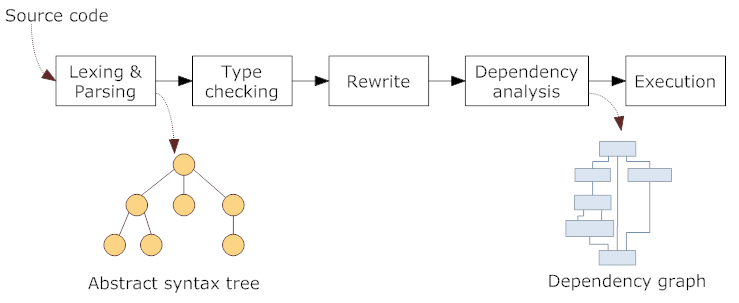
\includegraphics[width=0.8\textwidth]{phases.png}
  \caption{An overview of the analysis process.}
  \label{fig:phases}
\end{figure}

\subsection{Lexing and parsing}
\label{sub:lexing-parsing}

Lexing and parsing are two standard procedures in programming language
pragmatics. These two phases are responsible for what is usually
called ``syntactic analysis''. Ever since the first compilers were
written, syntactic analysis received a great deal of attention. Along
the years, this research produced a set of tools -- Lex and Yacc
\cite{lex-yacc} --, that has greatly simplified this task, to the
point where programming language researchers don't give it much
attention anymore, preferring to address theoretic foundations and
semantic concerns instead. As expected, EzQL uses these tools, which
means the biggest challenge in this phase was to guarantee that the
grammar was unambiguous, which is not much of a challenge these days.

\subsection{Type checking}
\label{sub:type-checking}

Type-checking -- including type-inference --, is implemented through
the well-known Damas-Milner algorithm\footnote{Out of curiosity,
  Lu\'{i}s Damas is a Portuguese researcher at the University of
  Porto.} \cite{damas-milner}. This algorithm works in two phases:
constraint collection and unification.

The first phase consists in performing a pass over the abstract syntax
tree produced by the parser and collecting a set of typing
constraints. For example, the following listing taken from the
previous chapter,

\begin{lstlisting}
  def printEvents (s, fn) =
      when ev in s -> print (fn(ev))
\end{lstlisting}

produces the following constraints:

\begin{enumerate}
\item \verb=printEvents= is a function that receives two parameters
  with initial types \verb='s= for the type of \verb=s= and \verb='f=
  for the type of \verb=fn=, and returns some other unknown type
  \verb='r=;
\item While it analyzes the \verb=when=, the type checker infers that
  the type of \verb=s= -- \verb='s= -- must be \verb=stream<'a>= for
  some event type \verb='a=. Also, the type of \verb=ev= must be
  \verb='a=;
\item Since \verb=fn= is called with \verb=ev=, \verb=fn= must be a
  function that receives an \verb='a= and returns some other type
  \verb='t=;
\item \verb=print= is a primitive function that receives anything and
  returns \verb=unit=, which means nothing. \verb=unit= plays a
  similar role to \verb=void= in C-like languages;
\item The return type of the entire \verb=when= expression must be the
  same as the return type of \verb=print=;
\item Finally, the return type of the entire function -- \verb='r=,
  must be the same as the return type of the \verb=when= expression,
  because there is nothing following the \verb=when=.
\end{enumerate}

Note that, at this point, the algorithm does not try to solve these
constraints, no matter how trivial the solution seems to be. This
happens only in the second phase, where the unification algorithm
tries to find consistent types for all terms. For the constraints
above, the algorithm finds out that:

\begin{itemize}
\item \verb=s= is of type \verb=stream<'a>=. Since there are no
  constraints regarding the type of the events in \verb=s=, the
  algorithm settles on the generic \verb='a= type, which essentially
  means ``accept any stream'';
\item \verb=fn= is a function that receives an \verb='a= and returns a
  \verb='r=. The return type has not been constrained because
  \verb=print= is a polymorphic function that accepts anything;
\item Finally, since \verb=print= returns \verb=unit=, so does
  \verb=when= and so does \verb=printEvents=. Thus, \verb=printEvents=
  accepts a \verb=stream<'a>=, a function from \verb='a= to \verb='r=
  and returns \verb=unit=.
\end{itemize}

Note that there is an implicit constraint between \verb=s= and
\verb=fn=, because they both reference the type \verb='a=. This means
that the type checker will guarantee that all calls to
\verb=printEvents= use consistent arguments. For example, the
following snippet would be refused:

\begin{lstlisting}
  stocks = stream of { timestamp:int, symbol:string, price:float }

  def not (b) =
    if b then false else true

  printEvents (stocks, not)
\end{lstlisting}

For this particular application, the type checker will try to replace
\verb='a= with the type of the events in the stream --
\verb={ timestamp:int, symbol:string, price:float }= which is not
consistent with the type of \verb=not=, which expects a simple
\verb=bool=.

\subsection{Rewriting phase}
\label{sub:rewriting}

Rewriting transforms the abstract syntax tree in order to lighten the
work that needs to be done by the remaining phases. In particular, it
takes most of the syntactic sugar that was added to make the language
more user-friendly -- but contains no semantic value whatsoever --,
and replaces it with more primitive constructs. It is interesting to
analyze a few transformations, to see how the runtime relies on these
primitives to implement higher-level features:

\begin{description}
\item[Function definitions] are transformed into simple variable
  definitions with anonymous function values:

  \begin{lstlisting}
    def not (b) =
      if b then false else true
  \end{lstlisting}

  is transformed into:

  \begin{lstlisting}
    not = fun b -> if b then false else true
  \end{lstlisting}

\item[Entity definitions] including associations, are transformed into
  \verb=group by= expressions, as alluded in section
  \ref{sec:entities};
\item[SQL-syntax] is transformed into an alternative ``method call''
  syntax more familiar to OOP programmers that we have not presented
  yet. For example, the following listing taken from section
  \ref{sec:streams-windows}

  \begin{lstlisting}
    from ev in stocks
    where ev.symbol == "ACME"
    select { price_x2 = ev.price * 2 }
  \end{lstlisting}

  is equivalent to:

  \begin{lstlisting}
    stocks
      .where  (fun ev -> ev.symbol == "ACME")
      .select (fun ev -> { price_x2 = ev.price * 2 })
  \end{lstlisting}

  While it seems less user-friendly, this syntax is more explicit and
  shows operators for what they really are: methods of the
  \verb=stream= class. In the case of \verb=where= and \verb=select=
  it also shows that the predicate and the projector are actually
  anonymous functions passed as parameters to these methods. This is
  interesting because if the developer is, somehow, allowed to
  implement these methods in EzQL, he will be able to create new
  operators without modifying the syntax of the language. More on this
  in chapter \ref{chap:eval}.

\end{description}

\subsection{Dependency analysis}
\label{sub:dataflow}

EzQL programs are composed by a number of definitions, or queries. The
results of these queries may be stored in variables and used by other
queries. As we have seen in chapter \ref{chap:ezql}, when a variable
is updated, its changes are propagated downward, so that other queries
that depend on it may be immediately updated too. This process
continues until there are no more changes left to spread. Furthermore,
it is not enough to simply propagate these changes -- we must do it in
the correct order too. To see why, suppose you have the following
definitions:

\begin{lstlisting}
  acmePrice = acmeStocks.last().price # current ACME's price
  xptoPrice = xptoStocks.last().price # current XPTO's price
  sumPrices = acmePrice + xptoPrice
\end{lstlisting}

Here, \verb=acmeStocks= contains only price reports from the financial
market related to ACME while \verb=xptoStocks= contains
XPTO's. Suppose a new event arrives into \verb=acmeStocks=: first
\verb=acmePrice= should be updated, and then \verb=sumPrices=. Now
suppose that, at the same time, new events arrive on both the
\verb=acmeStocks= and \verb=xptoStocks= streams: the system must
update both \verb=acmePrice= and \verb=xptoPrice= before it updates
\verb=sumPrices=.

To propagate values the right way, the engine performs some dependency
analysis over the code, which results in a dependency graph. This
graph also records the operators that should be used for each step of
the query, a characteristic it shares with query plans. An example of
this analysis is shown next, where the code below gives origin to the
graph in figure \ref{fig:graph1}.

\begin{lstlisting}
  stocks = stream of { timestamp:int, symbol:string, price:float }

  # For each company, calculates the ratio between the current price
  # and the maximum price of all companies.
  ratioOverMax =
    from ev in stocks
    group by :symbol into events
    select
      let currPrice = events.last().price
      let maxPriceOverall = stocks.max(:price)
      currPrice / maxPriceOverall
\end{lstlisting}

\begin{figure}[t]
  \centering
  \subfloat[Main graph]{\label{fig:graph1}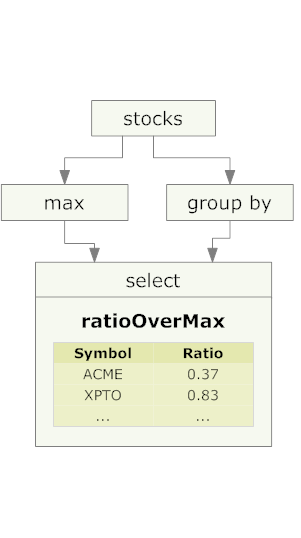
\includegraphics[width=0.25\textwidth]{ratioMax.png}}
  \subfloat[Main graph with select's inner graph]{\label{fig:graph2}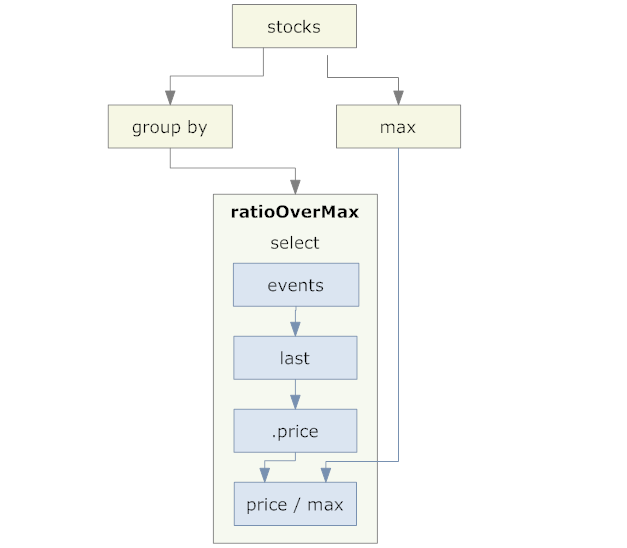
\includegraphics[width=0.5\textwidth]{ratioMax-expanded.png}}
  \caption{Dependency graph for \tt{ratioOverMax}}
\end{figure}


This example takes, once again, the \verb=stocks= stream and
calculates, for each company, the ratio between its current price and
the maximum price overall (not necessarily from the same company). In
the resulting graph we can see that the calculation of
\verb=maxPriceOverall= -- through the \verb=max= operator -- has been
taken out of the \verb=select=, which is allowed because it doesn't
depend on \verb=events=. On the other hand, the maximum becomes a
parent of \verb=select=, which makes sense: if the maximum changes, we
want \verb=ratioOverMax= to be immediately re-evaluated.

This raises an interesting question: to re-calculate the ratio of all
companies we will need the current price of each one of them. In some
cases however, this price may have been set by an event that arrived
minutes or even hours ago. Thus, in order to execute this query, the
system must store the current price of each company. How does it know
which values to keep?

The answer is that \verb=select= contains an inner graph that tells it
which operators are needed to execute the projection and which values
must be kept, as shown in figure \ref{fig:graph2}. This graph starts
with \verb=events=, which represents a stream with the events for each
group, and flows down to the node that is responsible for calculating
the final result (labeled \verb=price/max=). Note that the maximum
price is defined in the outer graph, but referenced by the inner
graph. This hierarchical structure may be extended for many more
levels. The following example illustrates this:

\begin{lstlisting}
  wereThere =
    from room in Room.all
    select (from product in Product.all
            where (product.room == room)[5 min].any?()).count()
\end{lstlisting}

\begin{figure}[t]
  \centering
  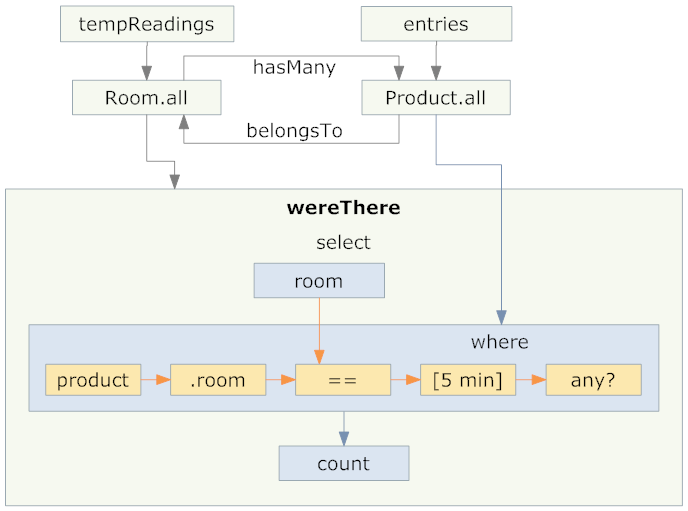
\includegraphics[width=0.6\textwidth]{wereThere.png}
  \caption{Dependency graph for \tt{wereThere}}
  \label{fig:graph-wereThere}
\end{figure}

This creates a dictionary that contains, for each \verb=Room=, the
number of products that were there at any moment during the last 5
minutes. The entire graph is shown in figure
\ref{fig:graph-wereThere}. As we can see, \verb=where= also has an
internal graph that is necessary to keep the 5 minutes window and the
result of the \verb=.any?()= aggregator. The interesting part is that
this internal graph references \verb=room=, which is part of the
\verb=select='s graph, which also references \verb=Product.all=,
defined in the outer scope. Whenever a product switches rooms,
\verb=Product.all= will propagate that change down to the
\verb=where=, the predicate will be updated and so will the
\verb=count()=. This culminates with the update of the \verb=select=,
whose result will be kept in \verb=wereThere=. Besides changes to
products, the five minutes windows, buried inside graphs of graphs as
they are, may ignite the update process, at any moment, due to the
expiration of some event. Moreover, if two of these things happen at
the same time, we will have two updates in parallel, which the system
must handle carefully in order to avoid messing up the results. All
this, however, happens during execution, which is the topic of the
next section.

\subsection{Execution}
\label{sub:execution}

After the dependency analysis is complete, the engine uses the graph
to create a network with the operators that will compute the results
during execution. Much like graph nodes may contain inner graphs, this
network's operators may also contain inner-networks. For example, the
\verb=where= operator uses its inner-graph to create an inner-network
for each entry that is added to the dictionary. This inner-network is
used to keep historic data necessary to calculate the result of the
predicate. This means the network is dynamic: when a new entry is
added to the dictionary, a sub-network is created just for it. Figure
\ref{fig:network} illustrates this.

\begin{figure} \centering
  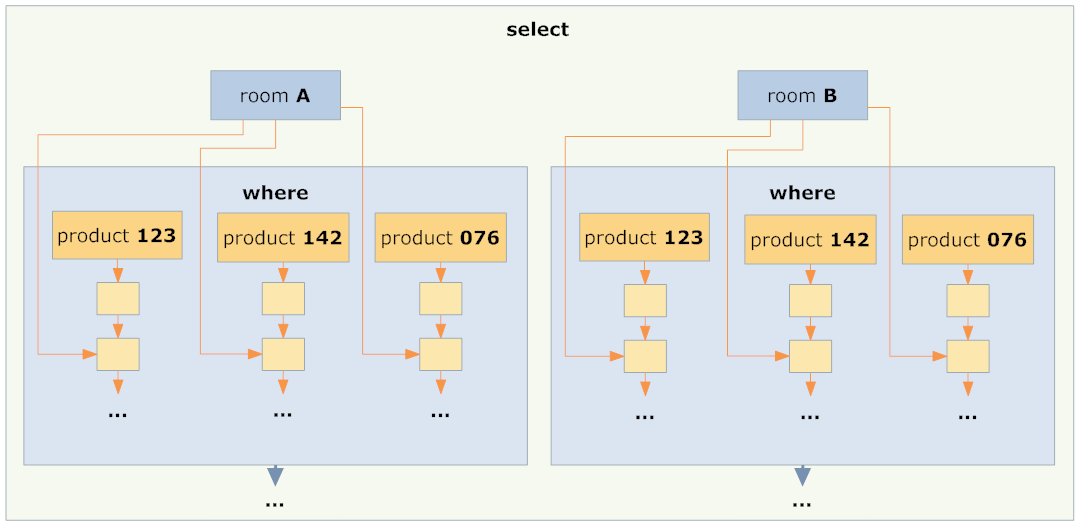
\includegraphics[width=0.8\textwidth]{network.png}
  \caption{During execution, the select and where operators for
    dictionaries replicate their sub-networks for each entry in the
    dictionary they are applied to. In this example, there are two
    rooms -- A and B -- and three products -- 123, 142 and 076 -- in
    the system.}
  \label{fig:network}
\end{figure}


Given that in EzQL queries run forever, the operators don't pass
complete results to each other. Instead, they communicate by sending
incremental changes. For example, when an event is added to a window,
the update signal that is propagated contains only the event, not the
entire window. Similarly when a new entry is added to a dictionary,
the dictionary propagates a change saying that the value at the given
key was updated. Moreover, these changes may be recursive. For
example, if the values of the dictionary are windows (which is allowed
in EzQL), the changes propagated by the dictionary contain the changes
propagated by the windows, and so on.

There are a total of 34 operators implemented in this prototype. They
can be classified into:

\begin{description}
\item[Stream and window operators], including the operators that
  represents a stream and a window, \verb=select= and \verb=where= for
  streams and windows, \verb=groupby=, \verb=when=, \verb=changes=,
  \verb=last= and \verb=sort=;
\item[Dictionary operators] corresponding to \verb=select= and
  \verb=where= for dictionaries, as well as \verb=values=;
\item[Aggregators], including: \verb=count=, \verb=sum=, \verb=avg=,
  \verb=min=, \verb=max=, \verb=any?=, \verb=all?=, \verb=howLong=;
\item[Other operators] a category that includes operators to represent
  function calls, records, indexers into dictionaries, field
  projectors out of records and an operator that implements an
  interpreter and is capable of executing some simple expressions.
\end{description}

The freedom EzQL provides allows for some unexpected combinations of
these operators. Creating dictionaries of other dictionaries, opening
timed windows inside function definitions, storing streams inside
record fields, are some rather surprising combinations that EzQL does
not forbid. Coordinating all these operators and testing some of the
infinite ways one can join them together, consumed a major part of
this work. The single task of coming up with an architecture flexible
enough to support our requirements -- the need to create and destroy
operators during runtime, operators that may depend on other operators
situated in different networks, the handling of simultaneous events
and expirations -- took some thought to mature. Still, that is not the
end of the story.

\section{Complications on a scheme}
\label{sub:complications}

\subsection{Round and around}

The graph that is created by the dependency analysis cannot contain
cycles, otherwise the changes propagation algorithm may not
terminate. Fortunately, cyclic dependencies are forbidden by design: a
definition cannot reference other definitions declared below. There
is, however, an exception to this rule: the
\verb=belongsTo=/\verb=hasMany= combo may need to refer to an
undeclared entity. For example, in

\begin{lstlisting}
  entity Product =
    createFrom (entries, :productId)
    belongsTo :room

  entity Room =
    createFrom (tempReadings, :roomId)
    hasMany :products
\end{lstlisting}

\verb=belongsTo= refers to the \verb=Room= entity, which has not yet
been declared. This has consequences on two stages of the code
analysis: type checking and dependency analysis. The type checker will
fail because it can't find the type of the \verb=room= field that
\verb=belongsTo= adds to the \verb=Product= entity. The dependency
analysis algorithm, on the other hand, will fail because it can't find
the \verb=Room.all= dictionary which is a dependency of
\verb=Product.all=.

Our solution consists in performing a normal pass over the code. If an
undeclared reference is found, though, an exception is thrown and the
algorithm records the field that caused the problem and the unknown
reference. In the example above, the \verb=room= field created by the
\verb=belongsTo= would cause an exception, because the entity
\verb=Room= had not yet been declared. The algorithm would then
proceed as if the \verb=room= field did not exist. When \verb=Room=
had been analyzed, the algorithm would check if there were any pending
operations that depend on it and would find that \verb=Product= needed
to be re-checked, which it would do right away. This operation may
take a few iterations to complete if both entities depend on each
other in intricate ways (for example, if \verb=Room= needs the
\verb=room= field of any of its \verb=products=).

\subsection{Filter doesn't actually filter}

In section \ref{sub:associations} we alluded to a problem related to
filtered dictionaries and historic data used in predicates or
projections over them. This happened while discussing the following
example:

\begin{lstlisting}
  wereInRoomB =
    from p in Room.all["A"].products
    where (p.roomId == "B")[5 min].any?()
\end{lstlisting}

The \verb=where= predicate asks for the results of the condition
\verb!p.roomId == "B"! over the last 5 minutes, for all products that
are in room A. However, the system must keep this information for all
products -- not just for the ones in room A --, because, as far as the
system is concerned, a product may switch to room A at any moment, and
when it does, the 5 minutes history must be readily available.

The prototype copes with this situation by keeping data for the hidden
entries inside dictionaries. Thus, dictionaries contain both hidden
and visible entries and handle them the same way. When an hidden entry
is updated, its changes are propagated as usual, except they are
tagged as being hidden, so that other operators may keep them
invisible to the outside. For example, if the application tries to
index a hidden entry with \verb=wereInRoomB[<hiddenProductId>]=, the
result will be \verb=null=.


\section{Testing and validation}
\label{sec:testing}

In order to test the prototype and to verify it gives correct answers,
we developed a small testing library. This library tests the engine
using a black-box approach: it sends events into the input streams and
checks if the monitored operators react accordingly. Furthermore, if
an unexpected events occurs, a warning will be emitted.

Currently, the prototype comes with a test-suite encompassing about
140 test cases and more than 900 assertions.

\chapter{Evaluation}
\label{chap:eval}

In this chapter, we apply EzQL to some real-world event processing
problems and discuss how does it compare to solutions written in other languages.

\section{The ``too muggy query''}

This query was first introduced in section
\ref{sec:defective-products}, where we also presented and discussed a
solution implemented in Coral8 CCL. The equivalent program in EzQL is
as follows:

\begin{lstlisting}
tempReadings = stream of { roomId:int, temperature:int }
entries = stream of { roomId:int, productId:int }

entity Room =
  createFrom(tempReadings, :roomId)

entity Product =
  createFrom (entries, :productId)
  belongsTo :room
  member this.temperature = this.room.temperature

defective =
  from p in Product.all
  where (p.temperature > 25).howLong() >= 10 min
\end{lstlisting}

This example uses only operators shown in chapter \ref{chap:ezql} and
thus, should not be difficult to understand. We begin by declaring the
input streams, then we define the \verb=Room= and \verb=Product=
entities, and finally, we declare the ``too muggy'' query that solves
the problem.

One of the issues with the solution presented in section
\ref{sec:defective-products} is that it doesn't solve the entire
problem, because it ignores humidity. The following listing extends
the example above to support humidity:

\begin{lstlisting}
# input streams
tempReadings = stream of { roomId:int, temperature:int }
humReadings = stream of { roomId:int, humidity:int }
entries = stream of { roomId:int, productId:int }

tempsAndHums = merge(tempReadings, humReadings, :roomId)

# define the entities
entity Room =
  createFrom(tempsAndHums, :roomId)

entity Product =
  createFrom (entries, :productId)
  belongsTo :room
  member this.temperature = this.room.temperature
  member this.humidity    = this.room.humidity

# which products are defective?
defective =
  from p in Product.all
  where (p.temperature > 25 and p.humidity > 80).howLong() >= 10 min
\end{lstlisting}

We begin by declaring a new stream -- \verb=humReadings= --, which is
merged with \verb=tempReadings=. \verb=merge= is a simple operator
that receives events from two streams and joins them into one. Every
time an event arrives on any input stream, it is sent to the single,
output stream. However, if two events arrive at the same time on both
streams, \verb=merge= will try to join them if they share a common
field -- \verb=roomId= in this example. In other words, if
\verb=tempReadings= receives these events:

\begin{tabular}{ |l|l|c| }
  \hline
  \verb=timestamp= & \verb=roomId= & \verb=temperature= \\
  \hline
  11:00:00 am & \verb="A"= & 20 \\
  11:01:00 am & \verb="B"= & 29 \\
  \hline
\end{tabular}

and \verb=humReadings= receives these:

\begin{tabular}{ |l|l|c| }
  \hline
  \verb=timestamp= & \verb=roomId= & \verb=humidity= \\
  \hline
  11:00:00 am & \verb="C"= & 67 \\
  11:01:00 am & \verb="B"= & 73 \\
  11:02:00 am & \verb="A"= & 75 \\
  \hline
\end{tabular}

then \verb=merge(tempReadings, humReadings, :roomId)= will result in:

\begin{tabular}{ |l|l|c|c| }
  \hline
  \verb=timestamp= & \verb=roomId= & \verb=temperature= & \verb=humidity=\\
  \hline
  11:00:00 am & \verb="A"= & 20 & null \\
  11:00:00 am & \verb="C"= & null & 67 \\
  11:01:00 am & \verb="B"= & 29 & 73 \\
  11:02:00 am & \verb="A"= & null & 75 \\
  \hline
\end{tabular}

When the events are not merged -- either because there was only one
event or the events didn't match --, \verb=merge= fills the unknown
fields with \verb=null=. In EzQL, most operators on continuous values
ignore \verb=null=, which means that, for example, the temperature of
room A remains at 20 degrees at 11:02:00 am. Also, note that
\verb=merge= may put two different events with the same timestamp into
the same stream, which means EzQL demands support for simultaneous
events.

We use the result of merging both streams to instantiate the
\verb=Room= entity. Thus, every \verb=Room= instance will
automatically be equipped with \verb=temperature= and \verb=humidity=
field. We them use this last field to define the \verb=Product='s
humidity, much like we had done previously with the temperature. At
last, in the final line, we update the condition to take humidity into
account.

\section{Linear road benchmark}

The Linear Road benchmark \cite{lrb} was introduced as a first attempt
at producing a realistic benchmark for ESP engines. In \cite{cql}, the
creators of CQL implemented a simplified version to introduce their
language and discuss its semantics. This makes the linear road
benchmark of particular importance, because it allows us to compare
EzQL with CQL, using an example that, presumably, CQL handles well.

The benchmark itself models a road traffic management scenario with a
number of highways where the cost of traveling is calculated in
real-time and is dependent on the traffic conditions. Intuitively, a
costumer pays more if he chooses to drive by a congested segment,
because he is contributing for the increase in traffic inside that
segment. Hopefully, the common goal to pay less somehow drives
costumers to regulate traffic in a way that is beneficial for
everyone.

\begin{figure}[t]
  \centering
  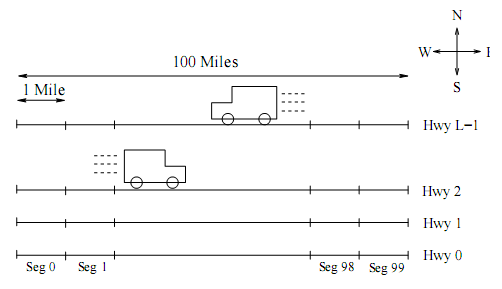
\includegraphics[width=0.6\textwidth]{lrb.png}
\caption{The linear-road highway system. Image taken from \cite{cql}}
\end{figure}


To simplify, we assume the highways run from east to west. All
vehicles report their position and velocity every 30 seconds to a base
station. The position is specified using three attributes: the highway
number, the direction (east or west) and the distance the vehicle is
from the western endpoint of the highway. A base station aggregates
this data to calculate the toll for each segment. For non-congested
segments, the toll is 0. For congested segments, on the other hand,
the toll is calculated using the formula \(basetoll * (numvehicles -
150)^2\), where \(baseToll\) is a constant parameter and
\(numvehicles\) is the number of vehicles currently in the
segment. Furthermore, a segment is considered to be congested if the
average speed of all vehicles in that segment over the last 5 minutes
is less than 40 mph. Finally, we assume that highways are 100 miles
long and are divided into one hundred 1-mile segments. Thus, the current
segment of a vehicle is defined by the triple (highway, direction,
xPos/1760). The input for this problem is a single stream with the
position and speed reports for all vehicles. We use this stream to
find an answer to our main problem: how much does each costumer pay in
the end?

The solution in CQL, taken from \cite{cql}, is transcribed in appendix
\ref{sec:lrb-cql}. The algorithm consists in applying successive
operations to the input stream to produce a few derived streams and
relations, which are then combined to compute the answer. Figure
\ref{fig:lrb-cql} shows how these derived streams and relations
interact with each other.

\begin{figure} \centering
  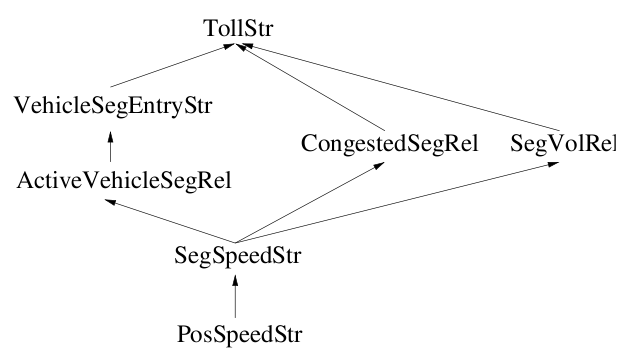
\includegraphics[width=0.5\textwidth]{lrb-cql.png}
  \caption{Derived streams and relations in the solution to the linear
    road benchmark. Image taken from \cite{cql}.}
  \label{fig:lrb-cql}
\end{figure}


The six queries are not difficult to understand by
themselves. However, the simple fact that the authors had to create a
diagram to explain their solution should raise an alarm. All these
temporary streams and relations show a symptom that we already
discussed in section \ref{sec:defective-products}: the only way to
manage complexity using existing languages is through the creation of
a large number of intermediary streams and windows, which are coupled
with each other in ways that violate most best-practices. A second
problem with this solution is related to time management. For example,
the last query outputs the toll for each vehicle that enters a
segment. We copy it here for easier reference:

\lstset{
  language=CCL,
  columns=fullflexible,
  basicstyle=\tt,
  keywordstyle=[1]\bf,
  keywordstyle=[2]\it,
}

\begin{lstlisting}
# Query 6: TollStr(vehicleId,toll)

Select Rstream(E.vehicleId,
               basetoll * (V.numVehicles - 150)
                        * (V.numVehicles - 150) as toll)
From VehicleSegEntryStr [Now] as E,
     CongestedSegRel as C, SegVolRel as V
Where E.segNo = C.segNo and C.segNo = V.segNo and
      E.dir = C.dir and C.dir = V.dir and
      E.hwy = C.hwy and C.hwy = V.hwy
\end{lstlisting}

\lstset{
  language=EzQL,
  columns=fullflexible,
  basicstyle=\tt,
  keywordstyle=[1]\bf,
  keywordstyle=[2]\it,
}

To control precisely when this query should be executed, an inner join
between three entities is performed, one of which is a stream that
signals the entry of a vehicle in a new segment. However, this is not
immediately obvious. We believe that developers should not need to
worry with the exact time a query is executed: that is a low level
detail that should be abstracted by the system. However, if the
problem requires such fine-grained control, there must be a better way
to do it than joining streams. A third and final problem with this
example pertains to the way the toll is calculated. In the last query,
the toll is calculated for each vehicle. However, this does not make
sense from a modeling point of view: the toll is an attribute of the
segment, not of the vehicle. This could probably be easily changed.
But the point is: CQL does not provide any means to enforce an
accurate modeling of the problem at hand, which reinforces our idea
that all these streams are only temporary and won't be used
extensively as a building-block for other queries.

The equivalent solution in EzQL is presented below:

\begin{lstlisting}
posSpeedStr = stream of { vehicleId:int, speed:int, hwy:int,
                             dir:bool, pos:int }

baseToll = 100 # any value will do

# Convert x coordinates to segment numbers
segSpeedStr =
  from ev in posSpeedStr
  select { vehicleId = ev.vehicleId, speed = ev.speed,
           segmentId = (ev.hwy, ev.dir, ev.pos / 1760) }

entity Segment =
  createFrom(segSpeedStr, :segmentId)
  hasMany :vehicles

  # A segment is congested if the speed average reported over the
  # last 5 minutes is less than 40 mph
  member this.isCongested =
    let avg5mins = this.events[5 min].avg(:speed)
    if avg5mins.null?
      then false
      else avg5mins < 40

  # The toll for this segment
  member this.toll =
    if this.isCongested
      then baseToll * (this.vehicles.count() - 150) ^ 2
      else 0

entity Vehicle =
  createFrom(segSpeedStr, :vehicleId)
  belongsTo :segment

  member this.amount = 0
    when this.segmentId.changes() -> this.amount + this.segment.toll


# amount per vehicle
amountPerVehicle =
  from v in Vehicle.all
  select v.amount
\end{lstlisting}

We begin by converting the position coordinates sent by the vehicles
into segment numbers. Note that the \verb=segmentId= field is a triple
containing the highway number, the direction and the segment number.
Then, we use the resulting stream to define the \verb=Segment= and
\verb=Vehicle= entities. We then define the \verb=isCongested= member,
that checks if a \verb=Segment= is congested. It does so by getting
the average speed over the last 5 minutes in the \verb=this.events=
member. As explained in chapter \ref{chap:ezql}, \verb=events= is a
stream created automatically by \verb=createFrom= that contains all
the events related to this segment. If there were no cars in this
segment during that interval, the segment is not congested for
sure. Otherwise, it is congested only if the average is below 40
mph. We then proceed by calculating the current toll for each segment,
using the formula given above. For the \verb=Vehicle= entity we define
the single attribute \verb=amount= that starts at 0, but is
incremented by the current segment's toll every time the vehicle
changes to a different segment. Finally, the last few lines declare a
query that obtains, for all vehicles, the amount they have to pay.

How does our solution compare to the one written in CQL? For starters,
instead of defining several streams and relations, we model the
scenario by declaring two queries and defining two entities. These
entities group several members together that may be seen as attributes
of their instances. This is an important difference, because when the
developer adds a new member to an entity, he is somehow forced to
think ``does this make sense?''  or ``will this interfere with the
work of my coworkers?''. Intermediate streams, on the other hand, are
used in isolation, as local variables in a procedure. Hence, most
developers don't really care if these streams could be reused or if
they model the scenario accurately, which means they will become
forgotten after a couple usages.

Another important difference is that we use when blocks to specify
\emph{when} the amount to pay be should updated. In our opinion, this
is clearer than joining streams and windows.

% TODO: Say that it is shorter (but is it?)

%\begin{figure}[htbp]
%  \centering
%  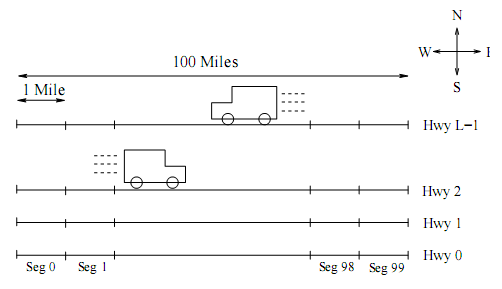
\includegraphics[width=\textwidth]{lrb.png}
%  \caption{Dependency graph for the Linear Road benchmark.}
%  \label{fig:eventflow-sample}
%\end{figure}



\section{Stock data analysis}

In this section we implement a few common financial market analysis
indicators that may be used to support the trading decision
process. The reader is advised not to adventure himself into this
hostile market armed solely with these primitive algorithms.

\subsection{MACD}

MACD \cite{macd-book} -- or Moving Average Convergence/Divergence --,
is a financial market indicator created by Gerald Appel that may be
used to predict the right time to sell or buy stocks from some
company, using only the past evolution in their prices. Its
calculation is very simple:

\begin{enumerate}
\item First, we calculate the exponential moving average (EMA) of the
  prices over the last 12 and 26 days (these numbers are only
  recommendations) and subtract them. This gives us the \emph{MACD};
\item Then, we obtain another exponential moving average over the MACD
  itself, regarding the last 9 days. This gives us the \emph{signal}.
\end{enumerate}

Figure \ref{fig:macd} shows all these values plotted against the price
of some company's stocks. We can now subtract the MACD by the signal
to find out, using a very primitive algorithm, if we should be buying
or selling stocks from that company. If the MACD becomes greater than
the signal, we should buy. Otherwise, if the MACD goes below the
signal, we should sell.

\begin{figure}[t]
  \centering
  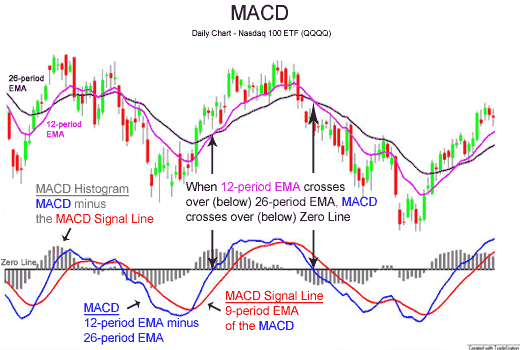
\includegraphics[width=0.6\textwidth]{macd.png}
  \caption{Sample plot showing the evolution of some stocks, as well
    as both 12 and 26 EMAs (in pink and black), the MACD (in blue) and
    the signal line (in red). Image copied from \cite{macd-plot:www}.}
  \label{fig:macd}
\end{figure}

StreamBase, one of the leading event processing products in the
market, comes with a sample project that calculates the MACD, which
should make for an interesting comparison. The code, copied as is from
the sample, is shown in section \ref{sec:macd}. Our solution is as
follows:

\pagebreak
\begin{lstlisting}
stocks = stream of { timestamp:int, symbol:string, value:float }

# Produces an event every day, at midnight.
midnight =
  from ev in ticks
  where ev.timestamp % 86400 == 0

entity Company =
  createFrom (stocks, :symbol)

  # Yesterday's final value
  member this.yesterday = 0.0
    when midnight -> this.value # value is created by createFrom

  member this.trend =
    let macd = ema(this.yesterday, 12) - ema(this.yesterday, 26)
    let signal = ema(macd, 9)
    macd - signal

  # Should we buy or sell stocks from this company?
  member this.buy = this.trend > 0
  member this.sell = this.trend < 0


toBuy =
  from c in Company.all
  where c.buy

when ev in toBuy.values().added() ->
  print("You should buy stocks from " + ev.value.symbol)
\end{lstlisting}

This snippet begins with the declaration of the \verb=midnight=
stream, using a variable that has not yet been introduced --
\verb=ticks=. This is a predefined stream that emits an event once per
second. \verb=midnight= filters all these events except one per
day. Thus, if the program begins execution at midnight, the stream
\verb=midnight= will actually output an event every day, at midnight,
thus notifying its users the day has changed. Naturally, it is not
realistic to demand this restriction in a real-world application, but
in this example it will do, as it is more or less orthogonal to the
calculation of the MACD.

Next, we define a \verb=Company= entity that has four attributes. The
first -- \verb=yesterday= --, contains yesterday's last price. Note
that this value is updated once per day. Thus, if we open a window
over it, we may get the closing prices of the previous days. The
second member -- \verb=trend= --, calculates the difference between
the MACD and the signal lines using the closing prices of the last few
days. Finally, \verb=buy= and \verb=sell= are simply the indicators we
want to monitor in order to make decisions.

At last, we declare a dictionary to contain all companies where the
\verb=buy= signal is enabled. In the final two lines, we monitor which
companies are added into this dictionary. These are the companies
where the MACD has just crossed the signal and, according to the
algorithm above, this is when we should be buying their stocks. As
discussed previously, the \verb=values()= operator returns a list with
the values in a dictionary. Using this list, we may then apply the
\verb=added()= operator to find out when a new entry is added into the
dictionary. There is also a corresponding \verb=expired()= operator that
signals the removal of an entry.

The example above uses the \verb=ema()= function to calculate the
exponential moving average. This is an user-defined aggregator
implemented in EzQL as follows:

\begin{lstlisting}
enum EmaState =
  | Init of { count:int, sum:float }
  | Normal of float

def ema(data, n) =
  let alpha = 2 / (n + 1.0)
  let result = Init ({ cnt = 0, sum = 0.0 })
    when data.changes() ->
      match result with
        | Init s ->
            if s.cnt < 2
              then Init ({ cnt = s.cnt + 1, sum = s.sum + data })
              else Normal ((s.sum + data) / (s.cnt + 1))
        | Normal f -> Normal (alpha * data + (1 - alpha) * f)

  match result with
    | Init s -> if s.cnt == 0 then 0 else s.sum / s.cnt
    | Normal f -> f
\end{lstlisting}

This code is complicated by the initialization: when there is no
history we can't calculate an EMA. Instead, we begin by calculating a
regular arithmetic mean. After 3 values are in, we switch to the real
EMA. This solution differentiates these two phases into two states
defined in \verb=EmaState=: \verb=Init= -- which contains a count and
a sum needed to calculate the mean -- and \verb=Normal= -- which
contains only the EMA's value. \verb=result=, which keeps this state,
begins in the \verb=Init= state with both \verb=sum= and \verb=cnt=
initialized at 0. When the value changes, if this is only the first or
second update, it updates the \verb=count= and \verb=sum= and remains
in the \verb=Init= state. If, on the other hand, this is the third
update, it switches into the \verb=Normal= state -- to never leave it
again -- using the arithmetic mean as the starting value.

This example illustrates how some more complex user-defined
aggregators may be implemented directly in EzQL. While the language
does not support, at the moment, any kind of module system, this
aggregator could be put into a standard library, so that it is readily
available to any developer, without having to re-implement it.

\subsection{Gainers \& losers}

Proceeding with our stock market scenario, we now set out to find out
which are the top gainers (losers) of today's session, that is, the
companies whose stocks have increased (decreased) the most, by
percentage, when compared to the closing price of the previous
day. Furthermore, we wish to use this information to categorize all
companies into 4 groups: high-gainers, small-gainers, small-losers and
high-losers. This is a possible solution:

\begin{lstlisting}
stocks = stream of { timestamp:int, symbol:string, value:float }

# Produces an event every day, at midnight.
# Assumes the program is started at midnight.
midnight =
  from ev in ticks
  where ev.timestamp % 86400 == 0

enum GainerState =
  | HighGainer
  | SmallGainer
  | SmallLoser
  | HighLoser



entity Company =
  createFrom (stocks, :symbol)

  # Yesterday's final value
  member this.yesterday = 0.0
    when midnight -> this.value

  # How much is the company gaining today
  member this.gain =
    let y = this.yesterday
    if y != 0.0
      then (this.value - y) / y
      else 0.0

  # Which state am I in?
  member this.gainerState =
    if this.gain > 0.03 then        # Gaining more than 3%
      HighGainer ()
    else if this.gain >= 0 then     # Just gaining
      SmallGainer ()
    else if this.gain > -0.03 then  # Losing less than 3%
      SmallLoser ()
    else                            # Losing a lot
      HighLoser ()
\end{lstlisting}

Using this information, we can, for example, find out who is the top
gainer:

\begin{lstlisting}
topGainer = Company.all.values().sortBy(:gain)[-1]
\end{lstlisting}

\verb=sortBy()= sorts the list it is given by the \verb=gain= field,
while \verb=[-1]= accesses the last element of this sorted list, which
is our top gainer.

We can also find out how long has each company spent in the
\verb=HighLoser= state:

\begin{lstlisting}
duration =
  from c in Company.all
  select (c.gainerState == HighLoser ()).howLong()
\end{lstlisting}

Finally, we may have an interest for companies that were losing a lot
sometime in the last 3 days but are now in the high gainers:

\begin{lstlisting}
interestingCompanies =
  from c in Company.all
  where
    let beenLosing = (c.gainerState == HighLoser ())[3 days].any?()
    beenLosing and (c.gainerState == HighGainer ())
\end{lstlisting}

\section{Vehicle tracking using GPS coordinates}

And now for something completely different. The FBI is working on a
drug case involving several mobsters, including Vito Soprano, Tony
Corleone and Larry David. Inspector Harry Callahan has managed to
attach a GPS transmitter on their cars. The plan is to discover the
places where the bosses meet in order to bug them (they are extremely
cautious and always meet outside, in isolated and open spaces). To
solve this problem, the FBI called EzQL expert Ellen Ripley that came
up with the following solution:

\begin{lstlisting}
gps = stream of { timestamp:int, vehicleId:int, lat:float, lon:float };;

# Some value copied from http://xkcd.com/10/
pi = 3.14159265

# Convert from degrees to radians
def deg2rad deg =
  deg * pi / 180.0

# Convert from radians to degrees
def rad2deg deg =
  deg * 180.0 / pi

# Converts from geographical to cartesian coordinates
def geo2cart (lat, lon)  =
  let (latr, lonr) = (deg2rad lat, deg2rad lon)
  (cos latr * cos lonr, cos latr * sin lonr, sin latr)

# Calculates the distance between two positions (in km).
def distance((lat1, lon1), (lat2, lon2)) =
  let theta = lon1 - lon2
  let d1 = sin (deg2rad lat1) * sin (deg2rad lat2) + cos (deg2rad lat1)
             * cos (deg2rad lat2) * cos (deg2rad theta)
  let d2 = acos d1
  let d3 = rad2deg d2
  d3 * 60.0 * 1.1515 * 1.609344

# Calculates the center of mass for all positions in the given window.
# See http://www.geomidpoint.com/calculation.html for an explanation.
def centerOfMass(positions:[(float, float)]) =
  # These are the accumulators
  let (tx, ty, tz, tt) = (0.0, 0.0, 0.0, 0.0)
    when
      | ev in positions.added() ->
          let (x, y, z) = geo2cart (ev.value)
          (tx + x, ty + y, tz + z, tt + 1.0) # add to the accums
      | ev in positions.expired() ->
          let (x, y, z) = geo2cart (ev.value)
          (tx - x, ty - y, tz - z, tt - 1.0) # subtract from the accums

  # Divide the accumulators by the number of points
  let (x, y, z) = (tx / tt, ty / tt, tz / tt)

  # Convert back to geographical coordinates
  let lon = atan (y / x)
  let hyp = sqrt (x * x + y * y)
  let lat = atan (z / hyp)
  (rad2deg lat, rad2deg lon)


entity Vehicle =
  createFrom (gps, :vehicleId)
  member this.pos = (this.lat, this.lon)


# Calculates the center of mass of all vehicles
center =
  let positions =
    from v in Vehicle.all
    select v.pos
  centerOfMass(positions.values())


# Have the vehicles been together for the past 5 minutes?
# We consider that they are together if they are less than 50
# meters away from the center of mass.
beenTogether_5min =
  # Are they together now?
  let allTogetherNow =
    from v in Vehicle_all
    select (distance (v.pos, center) < 0.05).values().all?()
  # Have they been together for the past 5 minutes?
  allTogetherNow[5 min].all?()
\end{lstlisting}

The first half of this solution consists in the definition of a few
functions. These are all just direct translations from mathematical
formulas. The only one that might be more difficult to understand is
\verb=centerOfMass()=, which receives a list with latitude and
longitude pairs. When a new pair is added into this list, we convert
the latitude and longitude to cartesian coordinates and add these
values to a few accumulators (\verb=tx=, \verb=ty= and \verb=tz=). If,
on the other hand, a pair is removed from this list, we subtract their
coordinates from the accumulators. Then, to calculate the center of
mass, we just divide these accumulators by the number of points (in
\verb=tt=) and convert back to geographic coordinates.

We use this function to calculate the center of mass of all vehicles
in the definition of \verb=center=. Finally, we check if all vehicles
are within 50 meters of the center of mass and remain so for at least
5 minutes.

\section{Final thoughts}

Throughout this chapter we have applied EzQL to a few event processing
problems. For some of them, we have also presented corresponding
solutions in existing event processing languages. It is our opinion
that EzQL is more expressive than the ``competition'' and allows for
more readable and maintainable code. This wouldn't be possible without
features such as continuous values, entities, functions and the richer
operator set, which provide the basis for the creation of new
abstractions that simplify the resolution of problems.

It should also be clear from the examples above how convenient it is
to be able to implement new user-defined aggregators. The usual ones
-- \verb=min=, \verb=max=, \verb=count=, \verb=sum=, etc -- are simply
not enough to handle all kinds of problems in a natural way. Other
engines allow this kind of extension, but the developer must implement
the UDAs in external languages such as Java or C. For example, here is
how to implement \verb=avg= in Coral8 (taken from
\cite{coral8-integration-guide}, page 277):

\lstset{
  language=C,
  columns=fullflexible,
  basicstyle=\tt,
  keywordstyle=[1]\bf,
  keywordstyle=[2]\it,
  tabsize=8,
  tab=$\hspace{1pt}$
}

\begin{lstlisting}
typedef struct _AvgData {
    C8Int m_sum;
    int m_count;
} AvgData;

...

AvgData initial_data = { 0, 0 };
C8UInt size = 0;
struct AvgData *data_ptr = NULL;

/* Get state (if any) from previous calls. */
data_ptr = (AvgData*)C8GetState(ctx, &size);

// If there is no state from previous calls, then
// this is probably the first invocation and we must
// allocate memory.
if (data_ptr == NULL || (size != sizeof(AvgData))) {
    data_ptr = &initial_data;
}

/* Update the sum and count */
if (C8IsPositiveMessage(ctx)) {
    data_ptr->m_sum += C8GetInt(ctx, 0);
    data_ptr->m_count++;
} else {
    /* Negative message - a row just exited the window */
    data_ptr->m_sum -= C8GetInt(ctx, 0);
    data_ptr->m_count--;
}

/* Set the result */
C8SetOutputFloat(ctx, (C8Float) (data_ptr->m_sum) / data_ptr->m_count);

/* Save state */
C8SetState(ctx, data_ptr, sizeof(AvgData));
return;
...
\end{lstlisting}

Here is how to do the same thing in EzQL:

\lstset{
  language=EzQL,
  columns=fullflexible,
  basicstyle=\tt,
  keywordstyle=[1]\bf,
  keywordstyle=[2]\it,
  tabsize=8,
  showtabs=true,
  tab=$\hspace{1pt}$
}


\begin{lstlisting}
def count(n:['a]) =
  let acc = 0
    when | ev in n.added()   -> acc + 1
           | ev in n.expired() -> acc - 1
  acc

# Sum for int windows
def sum(n:[int]) =
  let acc = 0
    when | ev in n.added()   -> acc + ev.value
           | ev in n.expired() -> acc - ev.value
  acc

# Avg for int windows. Uses null if the window is empty
def avg(n) =
  let c = count (n)
  if c == 0 then null else sum(n) / c
\end{lstlisting}

Our solution implements \verb=avg()= on top of \verb=sum()= and
\verb=count()=, which we also show, for completeness.

Despite our belief that EzQL is a better language than existing
alternatives, one question remains to be answered: is it expressive
enough to handle bigger programs, with thousands of lines of code and
more complex queries? In our opinion, no, not at this stage. This is
due to various reasons, but the one that is probably more relevant is
the inability to create new data types -- in particular recursive data
types, such as lists and trees -- and define new operators on
them. Streams, windows and dictionaries should be enough to handle a
fair amount of problems, but the day will come when new
data-structures and operators are the appropriate answer to a more
complex question. In fact, we saw this happen while implementing the
examples above: many operators were added during this stage because it
made sense to do so. What about the countless operators that may be
useful for other problems? Should we modify the system every time we
want to use a new operator? This is not feasible. In our opinion, the
best compromise is to allow the developer to extend the default
operator set, using no more than pure EzQL.

The reason these remarks are not in the ``future work'' section, is
because there is already some work done in this area. In particular,
it is possible to define very simple stream operators such as
\verb=select= and \verb=where=. To show this, we begin by ditching
streams as we know them. Instead, we will define streams using only
enumerations and continuous values:

\begin{lstlisting}
enum Stream =
  | Event of 'a
  | NoEvent
\end{lstlisting}

That is, a stream can be in one of two states: \verb=Event=, meaning
the stream has received an event (the event may be of an arbitrary
type, as signaled by the generic variable \verb='a=); and
\verb=NoEvent=, which, as the name implies, means the stream is empty.

Now, here comes \verb=select=:

\begin{lstlisting}
def select (str, proj) =
  match str with
  | Event ev -> Event (proj(ev))
  | NoEvent -> NoEvent ()
\end{lstlisting}

This function receives a stream and a projector and then simply
applies pattern matching over the stream: if the stream is in the
\verb=Event= state, the result will also be a stream that carries the
same event, after being projected. Otherwise, the resulting stream
will be in the \verb=NoEvent= state. Note that, under this model,
streams are just continuous values. And, as explained in section
\ref{sec:functions}, when a parameter to a function changes, the
function is re-evaluated. Thus, when the stream switches between the
\verb=Event= and \verb=NoEvent= states, all calls to \verb=select=
will be re-evaluated, to update the resulting stream.

This function may be used as follows:

\begin{lstlisting}
stocks_x2 = select (stocks, fun ev ->
                                { timestamp = ev.timestamp,
                                  symbol    = ev.symbol,
                                  price_x2  = ev.price * 2 })
\end{lstlisting}

Given that \verb=select= has already been added into the language as a
built-in operator, the usefulness of implementing a function to do the
same thing may not be immediately obvious. However, this approach
could be used to implement any kind of operator, without having to
modify the ESP engine itself. Of course, the syntax is a little bit
uglier, but that is insignificant when compared to the practical
advantages of being able to extend the language in this
way. Unfortunately, as we said above, EzQL lacks some features that
would enable the developer to implement more complex
operators. Studying and integrating these features should be a topic
for further research.


\chapter{Conclusions and future work}
\label{chap:future-work}

The concept of \emph{abstraction} is one of the most important ones in
computer engineering. In this field, abstractions are methods that can
be employed to control the complexity of a system. They are
everywhere: a procedure is an abstraction -- in general, the caller
doesn't need to, and should not need to, know the details of its inner
workings --, and so are data structures, modules, APIs. The operating
system is a (very concrete) abstraction for all the low-level work it
relieves from user-level programs. TCP/IP is an abstraction as
well. Even DBMSs and SQL are abstractions.

Over the years, software engineers have learned the value of having
good abstractions in their code. Experience tells that such code is
more extensible, reusable, readable and maintainable. Bad
abstractions, on the other hand, lead to code with many
inter-dependencies that is hard to understand and harder to modify,
which results in its eventual abandonment. Only it may be too late.

Which role do programming languages play in this world? It is simple:
they are the tools that allow us to create new abstractions. Some put
their emphasis on functions, others prefer classes and objects, but
they all seek the same: to provide a powerful medium over which one
can express the best abstractions to solve any given problem. This is
probably the single most important point that must be taken into
consideration when comparing languages, not syntactic details.

Over the course of this work, we have tried to analyze whether
existing event processing languages possess the means to handle
increasingly complex -- but still realistic -- problems. What we have
found is that (1) the simplistic semantics employed by the systems are
inappropriate for many problems and this gets in the way of
developers, (2) the developer needs to spend a lot of effort handling
low-level details, and (3) the limited operator sets these languages
provide are not enough to attend some of the special needs of event
processing problems. All these problems are the result of having the
wrong abstractions -- or having no abstractions at all.

These findings have led us to create an alternative language which, we
believe, is better at handling more complex problems. This is due to
features such as continuous values, entities and a richer operator set
that allows more expressive solutions. Features such as user-defined
aggregators and functions, on the other hand, provide some extension
capabilities that are providential in order to develop better
abstractions to tackle new problems. This work is far from complete,
though.

\section{Future work}

Future work should proceed in three directions: enriching the
language, studying possible optimizations to speed up processing and
creating better developer tools.

First and foremost, new features should be added to the language, in
particular the ability to create complex data types, because this kind
of power is required to handle really difficult problems. Then, to
simplify the core language -- which would be advantageous later on --,
we could perhaps re-implement many of the now primitive data types and
operators, such as windows or \verb=group by=, using only EzQL. Other
features that would be welcome additions include a module system,
inheritance (and using it with the entity association mechanism) and
integration with traditional databases.

Second, we should begin to pay attention to an aspect that was
completely overlooked during this work: optimization. Being a
higher-level language with more features than existing ones, it is, at
the same time, more difficult to optimize EzQL code and easier to use
it in inefficient ways. On the other hand, event processing
applications bring some new optimization opportunities with a lot of
potential. For example, during execution there are many operators that
could be updated in parallel, using multiple threads. We already have
a dependency graph that shows how data flows downward. The next step
would be to analyze it in order to find disjoint paths that could be
worked out in parallel. Other optimizations to study include ways to
decrease memory usage by sharing data and, why not, compilation to
machine code.

Finally, in this age of integrated debuggers and code-completion, any
language will be largely ignored without good developer tools. In the
case of EzQL, more than a tool to write code, we believe that a
debugger allowing the user to peek at the state of his program during
execution -- setting up breakpoints, checking the value of an operator,
see what kind of changes are being propagated -- would be a major
productivity booster.


\bibliography{thesis}
\bibliographystyle{plain}

\appendix
\chapter{Solutions to a few problems}

This appendix contains solutions to some of the problems discussed in
chapter \ref{chap:simple-questions-complex-answers}. We can't claim
these are the best solutions nor the smallest, but they shouldn't be
too far away. We added a few comments to help the understanding of the
code.

\section{The ACME problem}
\label{sec:acme-problem-solution}

\lstset{
  language=CCL,
  columns=fullflexible,
  basicstyle=\tt,
  keywordstyle=[1]\bf,
  keywordstyle=[2]\it,
}


\begin{lstlisting}
-- Algorithm:
--
-- Keep two windows: one for the last 20 minutes of data, and another
-- with the newest event that is older than 20 minutes (i.e., the one
-- that expired last from the first window). Then, join both windows
-- (union would be better, but Coral8 doesn't support it) and get
-- the max of prices in any of the two windows.

create input stream StreamIn
schema (
   symbol string,
   price  float
);

-- Keep the events from the last 20 minutes.
create window Last20Mins
schema (
  symbol string,
  price  float
) keep 20 minutes
insert removed rows into Expired;

 -- Insert the events into the window.
insert into Last20Mins
select *
from StreamIn;

-- Keeps the previously expired event from Last20Mins (one per symbol)
create window Expired
schema (
  symbol string,
  price  float
) keep last per symbol;

-- For each symbol, store its max value over the last 20 minutes.
create window Result
schema (
  symbol string,
  result float
) keep last per symbol;

-- Join both windows and get the max of either of them
-- This would be prettier with UNION
--
-- Note: When events expire, this generates two events: one before
--       the expiration and another after.
insert into Result
select L.symbol,
       max(coalesce(max(L.price),0), coalesce(max(E.price),0))
from   Last20Mins as L full outer join Expired as E
         on L.symbol = E.symbol
group by L.symbol;
\end{lstlisting}

\section{The defective products problem}
\label{sec:defective-products-solution}

This is just a simplification of the original problem. In particular,
it doesn't handle humidity and assumes that rooms have a single
temperature sensor.

\begin{lstlisting}
-- Algorithm:
--
-- - Always maintain an explicit counter per product containing
--   the number of seconds the product spent at > 20 degrees.
--   This counter also contains the time the product was last
--   updated (last_update).
--
-- - When a product switches rooms, if the temperature in the
--   previous room was > 20, add now() + last_update to the
--   counter and replace the previous last_update with now();
--
-- - When the temperature in a room changes, if the previous
--   temperature was > 20, add now() + last_update to the
--   counter and replace the previous last_update with now();
--

create input stream entries
schema (
   product_id string,
   room_id string
);

create input stream temp_readings
schema (
   room_id string,
   temperature integer
);

-- Holds the last two entries per product
create window ProductRoom
schema (
   product_id string,
   room_id string
) keep 2 rows per product_id;

insert into ProductRoom
select *
from entries;

-- Holds the last two temp_readings per room
create window RoomTemperature
schema (
   room_id string,
   temperature integer
) keep 2 rows per room_id;

insert into RoomTemperature
select *
from temp_readings;

create local stream OnExit
schema (
   product_id string,
   old_room_id string
);

-- When a product leaves a room, generate an event containing the
-- product and the old room.
insert into OnExit
select entries.product_id, ProductRoom.room_id
from   entries left outer join ProductRoom
         on entries.product_id = ProductRoom.product_id
where  entries.room_id != ProductRoom.room_id;

create local stream OnTemperatureChange
schema (
   room_id string,
   old_temperature string
);

-- When the temperature changes, generate an event containing the
-- room and the old temperature
insert into OnTemperatureChange
select temp_readings.room_id, RoomTemperature.temperature
from   temp_readings left outer join RoomTemperature
         on temp_readings.room_id = RoomTemperature.room_id
where  temp_readings.temperature != RoomTemperature.temperature;

-- Per each product, maintain a counter with the time the product
-- spent above 20 degrees and the last time this counter was updated
create window ProductTemperatureCounter
schema (
   product_id    string,
   time_above_20 interval,
   last_update   timestamp
) keep last per product_id;

-- Initialize this counter
insert into ProductTemperatureCounter
select product_id, 0 seconds, now()
from entries
where room_id = "A";

-- Every time the product leaves the room, checks if the temperature
-- in the old room was > 20 and updates the counter of that product
insert into ProductTemperatureCounter
select E.product_id,
       if T.temperature > 20
         then time_above_20 + now() - C.last_update
         else time_above_20
       end,
       now()
from  OnExit as E, RoomTemperature as T,
      ProductTemperatureCounter as C
where E.old_room_id = T.room_id
        and E.product_id = C.product_id;

-- Every time the temperature changes, checks if the previous
-- temperature was > 20 and updates the counters of all the products
-- in that room
insert into ProductTemperatureCounter
select R.product_id,
       if T.old_temperature > 20
         then time_above_20 + now() - C.last_update
         else time_above_20
       end,
       now()
from  OnTemperatureChange as T, ProductRoom as R,
      ProductTemperatureCounter as C
where T.room_id = R.room_id
        and R.product_id = C.product_id;
\end{lstlisting}

\section{The Linear Road Benchmark in CQL}
\label{sec:lrb-cql}

\lstset{
  language=CQL,
  columns=fullflexible,
  basicstyle=\tt,
  keywordstyle=[1]\bf,
  keywordstyle=[2]\it,
}


\begin{lstlisting}
Query 1: SegSpeedStr(vehicleId, speed, segNo, dir, hwy)

  select vehicleId, speed, xPos/1760 as segNo, dir, hwy
  from PosSpeedStr

Query 2: ActiveVehicleSegRel(vehicleId, segNo, dir, hwy):

  select distinct L.vehicleId, L.segNo, L.dir, L.hwy
  from SegSpeedStr [range 30 seconds] as A,
        SegSpeedStr [partition by vehicleId rows 1] as L
  where A.vehicleId = L.vehicleId

Query 3: VehicleSegEntryStr(vehicleId, segNo, dir, hwy)

  select istream(*) from ActiveVehicleSegRel

Query 4: CongestedSegRel(segNo, dir, hwy)

  select segNo, dir, hwy
  from SegSpeedStr [range 5 minutes]
  group by segNo, dir, hwy
  having Avg(speed) < 40

Query 5: SegVolRel(segNo, dir, hwy, numVehicles)

  select segNo, dir, hwy, count(vehicleId) as numVehicles
  from ActiveVehicleSegRel
  group by segNo, dir, hwy

Query 6: TollStr(vehicleId, toll)

  select rstream(E.vehicleId,
                    basetoll * (V.numVehicles - 150)
                              * (V.numVehicles - 150) as toll)
  from VehicleSegEntryStr [now] as E,
       CongestedSegRel as C, SegVolRel as V
  where E.segNo = C.segNo and C.segNo = V.segNo and
         E.dir = C.dir and C.dir = V.dir and
         E.hwy = C.hwy and C.hwy = V.hwy
\end{lstlisting}


\section{MACD calculation in StreamSQL}
\label{sec:macd}

\lstset{
  language=StreamSQL,
  columns=fullflexible,
  basicstyle=\tt,
  keywordstyle=[1]\bf,
  keywordstyle=[2]\it,
}

\begin{lstlisting}
create input stream stocks (
    symbol string,
    price double,
    date timestamp
);
create output stream OutputAll;
create output stream OutputDELL;
create output stream OutputIBM;

create memory table SequenceTable
(
    sequence_name string,
    count int
) primary key(sequence_name) using hash;

create stream out__AddSequenceNumber_1;

insert into SequenceTable (sequence_name, count)
select "sequence" as sequence_name, 1 as count
from stocks
on duplicate key update
count = SequenceTable.count + 1
returning stocks.symbol as symbol,
          stocks.price as price, stocks.date as date,
          SequenceTable.count as count
into out__AddSequenceNumber_1;

create stream out__EMA_1 ;
select symbol as symbol,
       exp_moving_avg(price, 26,  0.0741) as EMaslow,
       exp_moving_avg(price, 12, 0.15385) as EMAFast,
       lastval(count) as count,
       lastval(date) as date,
       lastval(price) as price
from out__AddSequenceNumber_1[tuples valid always offset 0]
group by symbol
into out__EMA_1;

create stream out__ValidateEMA_1;
select * from out__EMA_1
where (notnull(EMaslow) && notnull(EMAFast)) into out__ValidateEMA_1;

create stream out__MACD_1;
select symbol as symbol,
       EMAFast as EMAFast,
       EMaslow as EMaslow,
       EMAFast - EMaslow as MACD,
       count as count,
       date as date,
       price as price
 from out__ValidateEMA_1
 into out__MACD_1;

create stream out__AggregateSignal_1;
select symbol as symbol, lastval(price) as price, lastval(MACD) as MACD,
       exp_moving_avg(MACD, 9, 0.2) as signal, lastval(date) as date
from out__MACD_1[tuples valid always offset 0]
group by symbol
into out__AggregateSignal_1;

select * from out__AggregateSignal_1
where notnull(signal) into OutputAll;

select * from OutputAll
where (symbol=="DELL") into OutputDELL;

select * from OutputAll
where (symbol=="IBM") into OutputIBM;


\end{lstlisting}


\end{document}

